
\chapter{Quark Gluon Analysis}
\label{ch:quark_gluon_analysis}

\newthought{As any dedicated reader} can clearly see, the Ideal of practical reason is a representation of, as far as I know, the things in themselves; as I have shown elsewhere, the phenomena should only be used as a canon for our understanding. The paralogisms of practical reason are what first give rise to the architectonic of practical reason. As will easily be shown in the next section, reason would thereby be made to contradict, in view of these considerations, the Ideal of practical reason, yet the manifold depends on the phenomena.


\section{Data Preprocessing}
\label{sec:q:data_preprocessing}

The data consists of \num{43} data files taken between \num{1991} and \num{1995} totalling \SI{3.5}{\giga\byte} (Data). Along with this comes \num{125} files based on Monte Carlo (MC) simulations (\SI{8.4}{\giga\byte}) and additional \num{42} MC-files with only $b$-quark events (MCb) simulated (\SI{2.1}{\giga\byte}). The data files which are in the form of \emph{Ntuples}, ROOT's data format \autocite{brunROOTObjectOriented1997}, are converted to HDF5-files by using uproot \autocite{ScikithepUproot2019}. While iterating over the Ntuples, some basic cuts are applied before exporting the data to HDF5. The first one being that the (center of mass) energy $E$ in the event has to be within $\SI{90.8}{\GeV} \leq E \leq \SI{91.6}{\GeV}$ to only use the $Z$ peak data. The second one being that the sum of the momenta $p_\mathrm{sum}$ in each event is $\SI{32}{\GeV} \leq p_\mathrm{sum}$ to remove any $Z \rightarrow \tau^+ \tau^-$ events. To ensure a primary vertex, at least two good tracks are required where a good track is defined as having \num{7} TPC hits and $\geq$ 1 silicon hit. Finally it is required that the cosine of the thrust axis polar angle, which is the angle between the trust axis and the beam, is less than or equal to \num{0.8} to avoid any low angle events since the detector performance worsens significantly in that region. These cuts were standard requirements for the ALEPH experiment.
% (P. Hansen, personal communication, December, 2019, XXX).

One last cut which was experimented with was the threshold value for \emph{jet matching}. The jet matching is the process of matching the jet with one of the final state quarks. The jet is said to be matched if the dot product of between the final quark momentum and the jet momentum is more than then threshold value. Higher thresholds means cleaner jets but at the expense of less statistics. A jet matching threshold of \num{0.90} was found to be a good compromise between purity and quantity where \SI{97.8}{\percent} of all 2-jet events are matched and \SI{96.7}{\percent} of all other jets were matched\sidenote{Compare this to \SI{98.5}{\percent} and \SI{97.8}{\percent} for a threshold of \num{0.85} or \SI{95.9}{\percent} and \SI{93.9}{\percent} for a threshold of \num{0.95}.}.  

The data structure is quite differently structured in the Ntuples compared to normal structured data in the form of tidy data \autocite{JSSv059i10}. The data is organized such that one iterates over each event where the variables are variable-length depending on the number of jets in the events; this is also known as \emph{jagged} arrays. The data is un-jagged\sidenote{Such that e.g. a 3-jet event will figure as three rows in the dataset.} before exporting to HDF5-format and only the needed variables are kept. This reduces the total output file to a \SI{2.9}{\giga\byte} HDF5-file for both Data, MC, and MCb.

The number of events for each number of jets can be seen in Table~\ref{tab:q:datasize_data} for the Data and in Figure~\ref{tab:q:datasize_MC} for the MC and MCb. 

\begin{margintable}
  \centering
  \begin{tabular}{@{}rrr@{}}
  {} &       jets &     events \\
  \midrule
  \num{2}     &  \num{2359738} &  \num{1179869} \\
  \num{3}     &  \num{3619290} &  \num{1206430} \\
  \num{4}     &   \num{854336} &   \num{213584} \\
  \num{5}     &    \num{52775} &    \num{10555} \\
  \num{6}     &      \num{510} &       \num{85} \\
  Total       &  \num{6886649} &  \num{2610523} \\  
  \end{tabular}
  \vspace{\abovecaptionskip}
  \caption{The dimensions of the dataset for the actual Data. The numbers in the jet columns are the number of events multiplied with the number of jets; e.g. $85 \cdot 6 = 510$.}
  \label{tab:q:datasize_data}
\end{margintable}

\begin{margintable}
  \centering
  \begin{tabular}{@{}rrr@{}}
  {} &       jets &     events \\
  \midrule
  \num{2}     &  \num{7293594} &  \num{3646797} \\
  \num{3}     &  \num{10780890} &  \num{3593630} \\
  \num{4}     &   \num{2241908} &   \num{560477} \\
  \num{5}     &    \num{103820} &    \num{20764} \\
  \num{6}     &      \num{588} &       \num{98} \\
  Total       &  \num{20420800} &  \num{7821766} \\  
  \end{tabular}
  \vspace{\abovecaptionskip}
  \caption{The dimensions for the MC and MCb datasets.}
  \label{tab:q:datasize_MC}
\end{margintable}

\FloatBarrier
\section{Explanatory Data Analysis} \label{sec:q:EDA}

Since the machine learning models are only trained on the three vertex variables \code{projet}, \code{bqvjet}, and \code{ptljet} -- see \autoref{ch:hep:particle_physcis_LEP} for a deeper introduction to these variables -- these variables will be the primary focus of this section. Given the fact that MC-simulated data exists, the truth of each simulated event is also known. This allows us visualize the difference between the different types of quarks. In the MC simulation each event are generated such that the type of quark, or \emph{flavor}, is known and assigned the variable \code{flevt}. The mapping from flavor to \code{flevt} is:
\begin{table}[h!]
  \centering
  \begin{tabular}{@{}rccccc@{}}
  Flavor: & $bb$ & $cc$ & $ss$ & $dd$ & $uu$  \\
  % \midrule
  \code{flevt}: & \num{5} & \num{4} & \num{3} & \num{2} & \num{1}  
  \end{tabular}
  \vspace{\abovecaptionskip}
  % \caption{The dimensions for the MC and MCb datasets.}
  % \label{tab:q:flevt}
\end{table}

In addition to knowing the correct flavor, we define that an event is \emph{$q$-matched} if one, and only one, of the jets are assigned to one of the quarks, one, and only one, of the jets are assigned to the other quark, and no other jets are matched to any of the quarks. We can then define what constitutes a $b$-jet: if it has \code{flevt} $= 5$, the entire event is $q$-matched, and the jet is matched to one of the quarks. Similarly we define $c$-jets only with the change that \code{flevt} $= 5$, and $uds$-jets with \code{flevt} $\in \{1, 2, 3\}$. A gluon jet is defined as an any-flavor event which is $q$-matched but the jet is not assigned to any of the quarks. Strictly speaking, this means that $g$-jet is not \SI{100}{\percent} certain of being a gluon, however, since the MC simulation does not contain this information this is the only option. Due to the $q$-match criterion this also means that some jets are assigned the label \q{non-$q$-matched} which is regarded as background. The distribution of different types of jets can be seen in Table~\ref{tab:q:flevt_overview} and shown as relative numbers in Table~\ref{tab:q:flevt_overview_percent_relative} in the appendix.

\begin{table}[h!]
  \centering
  \begin{tabular}{@{}rrrrrr@{}}
    {}    & \multicolumn{1}{c}{$b$} & \multicolumn{1}{c}{$c$} & \multicolumn{1}{c}{$uds$} & \multicolumn{1}{c}{$g$} & non-$q$-matched    \\ 
    \midrule
    2     & \num{2713454} &  \num{944380} & \num{2125900} &       \num{0} & \num{1509860} \\
    3     & \num{2433878} &  \num{964212} & \num{2129218} & \num{3365969} & \num{1887613} \\
    4     &  \num{326264} &  \num{156332} &  \num{336548} & \num{1012198} &  \num{410566} \\
    5     &   \num{10332} &    \num{5960} &   \num{12668} &   \num{54525} &   \num{20335} \\
    6     &      \num{42} &      \num{26} &      \num{52} &     \num{320} &     \num{148} \\
    \midrule
    Total & \num{5483970} & \num{2070910} & \num{4433012} & \num{4604386} & \num{3828522} \\
  \end{tabular}
  \caption{Number of different types of jets for MC and MCb. See also Table~\ref{tab:q:flevt_overview_percent_relative} in the appendix for relative numbers.}
  \label{tab:q:flevt_overview}
\end{table}

With the criteria defined above for what constitutes a specific type of jet the 1D-distributions for the three vertex variables is plotted in Figure~\ref{fig:q:vertex_variables}. For all three subplots the histograms are show with a logarithmic $y$-axis, all $b$-jets in blue, $c$-jets in red, $g$-jets in green and all jets in orange. In fully opaque color are shown the distributions for 2-jet events, in dashed (and lighter color) 3-jet events, and in semi-transparent 4-jet events. In the left subplot the \code{projet} variable is plotted where it can be seen that high values of \code{projet} tend to indicate $b$-jets. In the middle subplot \code{bqvjet} is plotted which shares many similarities with the \code{projet}-variables, including that high values indicate $b$-jets. In the right subplot the \code{ptljet} is plotted. This variable has many zeros in it which correlates with mostly with gluon\sidenote{Around \SI{98}{\percent} of all $g$-jets are zeros compared to $\sim \SI{82}{\percent}$ for $c$-jets and $\sim \SI{70}{\percent}$ for $b$-jets.} and large values are mostly due to $b$-jets. In general it is clear to se how the differences in distribution between the \num{2}-, \num{3}-, and \num{4}-jet events are minor, with the one exception of \num{2}-jet events which does not contain any gluons at all. 

\begin{figure}
  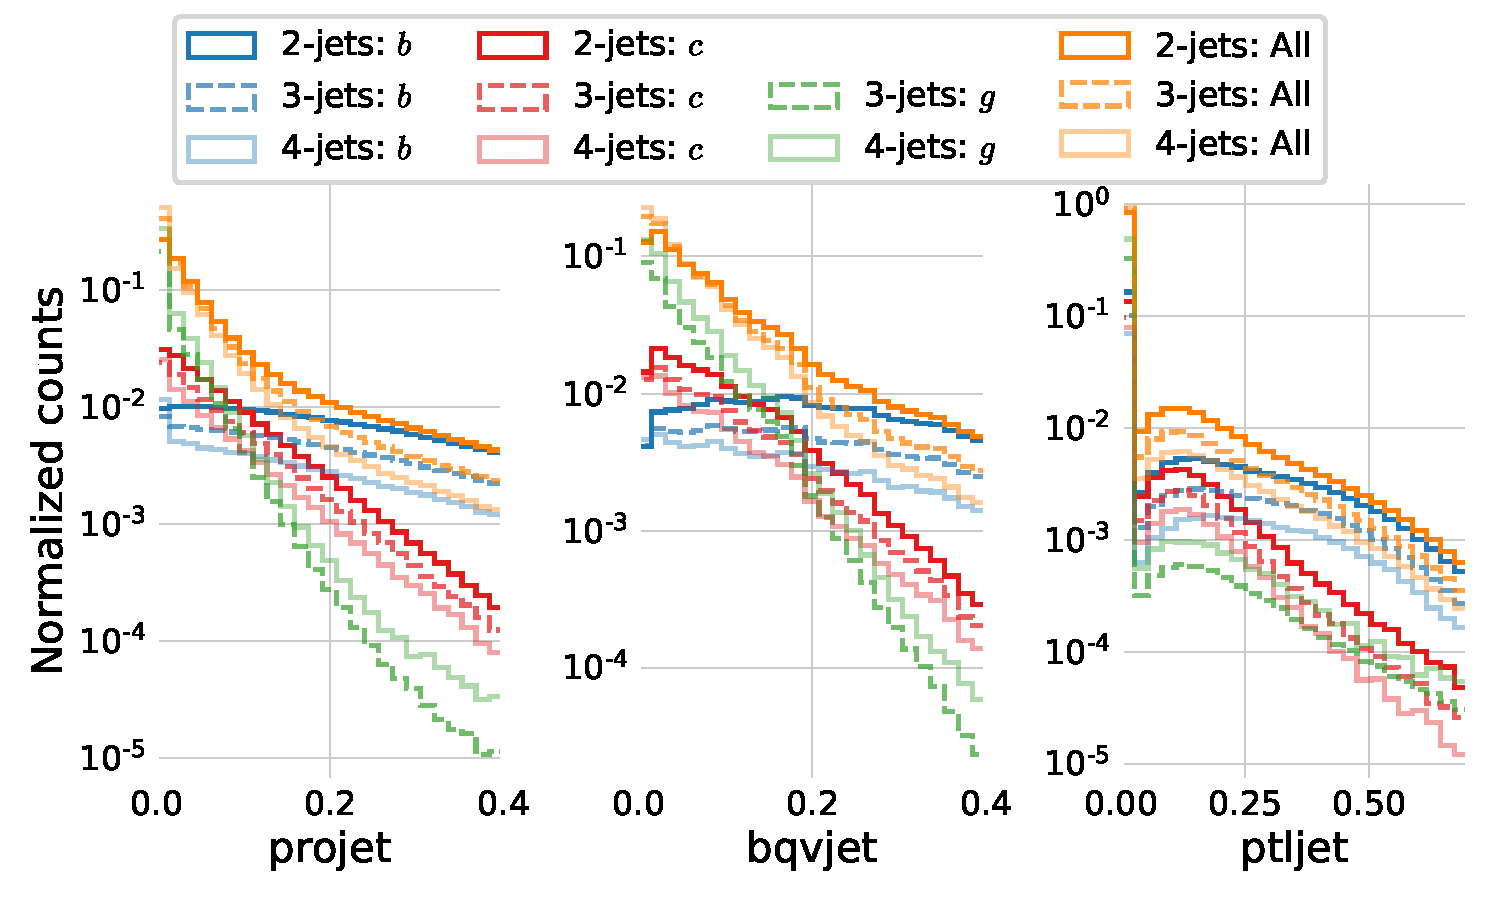
\includegraphics[width=0.98\textwidth, trim=0 0 0 0, clip]{figures/quarks/btagging_variables_hist-down_sample=1.00-ML_vars=vertex-selection=b-ejet_min=4-n_iter_RS_lgb=99-n_iter_RS_xgb=9-cdot_cut=0.90-version=19.pdf}
  \caption[Histograms of the vertex variables]
          {Normalized histograms of the three vertex variables: \code{projet}, \code{bqvjet}, and \code{ptljet}. In blue colors the variables are shown for \textcolor{blue}{true b-jets}, in red for \textcolor{red}{true c-jets}, in green for \textcolor{green}{true g-jets}, and in orange for \textcolor{orange}{all of the jets} (including non q-matched). In fully opaque color are shown the distributions for 2-jet events, in dashed (and lighter color) 3-jet events, and in semi-transparent 4-jet events. Notice the logarithmic y-axis, that there are no g-jets for 2-jet events (as expected), and that all of the distributions are very similar not matter how many jets.
          } 
  \label{fig:q:vertex_variables}
\end{figure}

Even though there are only three vertex variables, it is difficult to properly get an intuition about how easily separated they different types of jets are. Since there are millions of points a single 3D scatter plot quickly becomes overcrowded in one wants to plot all jets. We apply dimensionality reduction from the three dimensions down to two dimensions by using the UMAP algorithm \autocite{mcinnesUMAPUniformManifold2018}. Within recent years the field of dimensionality reduction algorithms has grown a lot from just the typical (linear) principal component analysis to also include non-linear algorithms. The t-SNE algorithm \autocite{maatenVisualizingDataUsing2008} deserves an honorable mention since this algorithm revolutionized the usage of (nonlinear) dimensionality reduction algorithms in e.g. bioinformatics \citep{toghieshghiQuantitativeComparisonConventional2019, wallachProteinSmallmoleculeDatabase2009}  yet its mathematical foundation has strongly been improved with the never, faster UMAP algorithm \autocite{mcinnesUMAPUniformManifold2018} which usage is also expanding \citep{bechtEvaluationUMAPAlternative2018, bechtDimensionalityReductionVisualizing2019, diaz-papkovichUMAPRevealsCryptic2019}.

The aim of UMAP, short for Uniform Manifold Approximation and Projection, is to correctly identify and preserve the structure, or topology, of the high-dimensional feature space in a lower-dimensional output space. It does so by trying to stitch together local manifolds in the high-dimensional feature space such that the difference between the high- and low-dimensional representations is minimized according to the cross-entropy such that both global structure and local structure is preserved \citep{mcinnesUMAPUniformManifold2018}. Compared to t-SNE the approach in UMAP has an algebraic topological background compared to the more heuristic approach taken by t-SNE. Note that the UMAP algorithm is not provided any information about which jets are which types. 

\begin{marginfigure}
  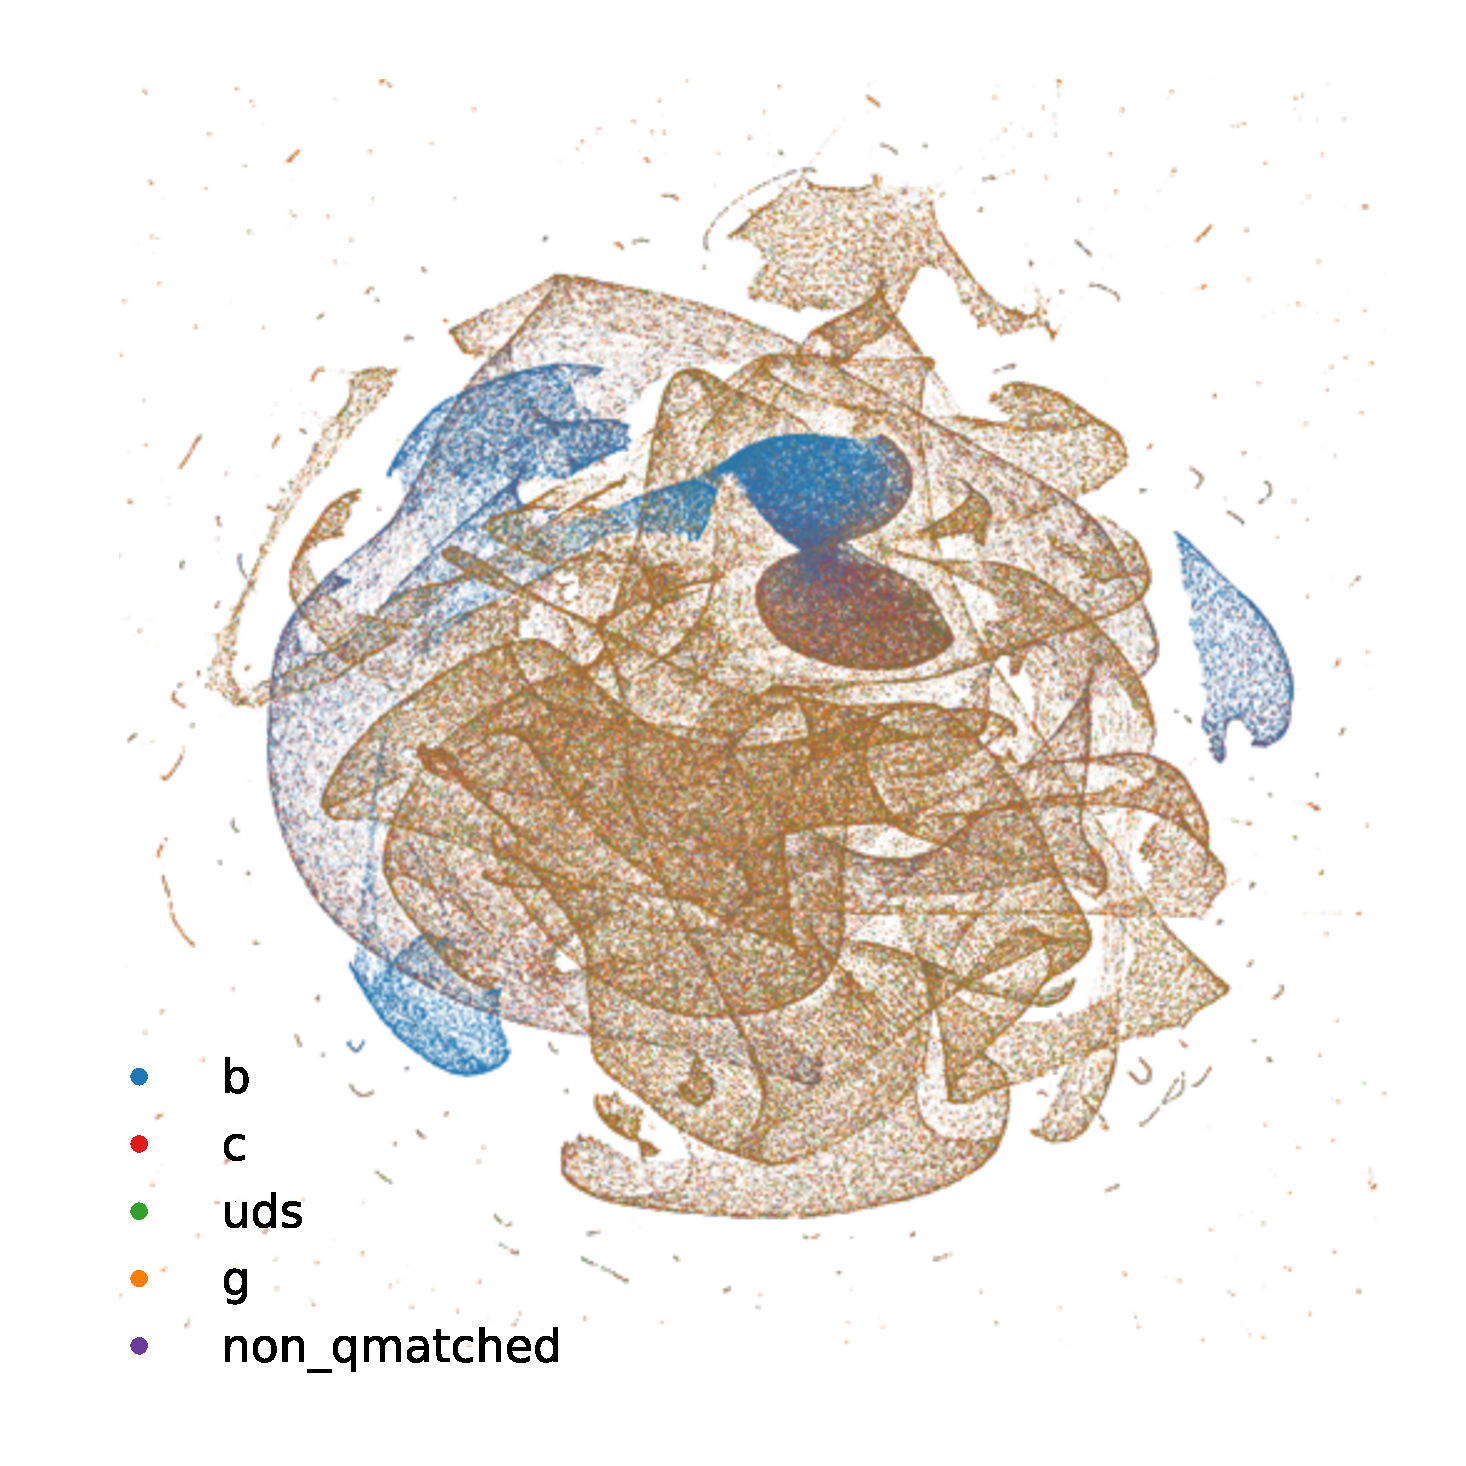
\includegraphics[draft=true, width=0.95\textwidth, trim=50 45 50 50, clip]{figures/quarks/df_UMAP-X=1120952-n_neighbors=250-min_dist=0.2-metric=euclidean-input2b_njet=4_algorithm=UMAP_single.pdf}
  \caption[UMAP visualization of vertex variables for 4-jet events]
          {Visualization of the vertex variables for the different categories: \textcolor{blue}{true b-jets} in blue, \textcolor{red}{true c-jets} in red, \textcolor{green}{true uds-jets} in green, \textcolor{orange}{true g-jets} in orange, and \textcolor{purple}{non q-matched} events in purple. The clustering is performed with the UMAP algorithm which outputs a 2D-projection. This projection is then visualized using the Datashader which takes takes care of point size, avoids over and underplotting, and color intensity.} 
  \label{fig:q:UMAP_vertex_2j}
\end{marginfigure}

\begin{marginfigure}
  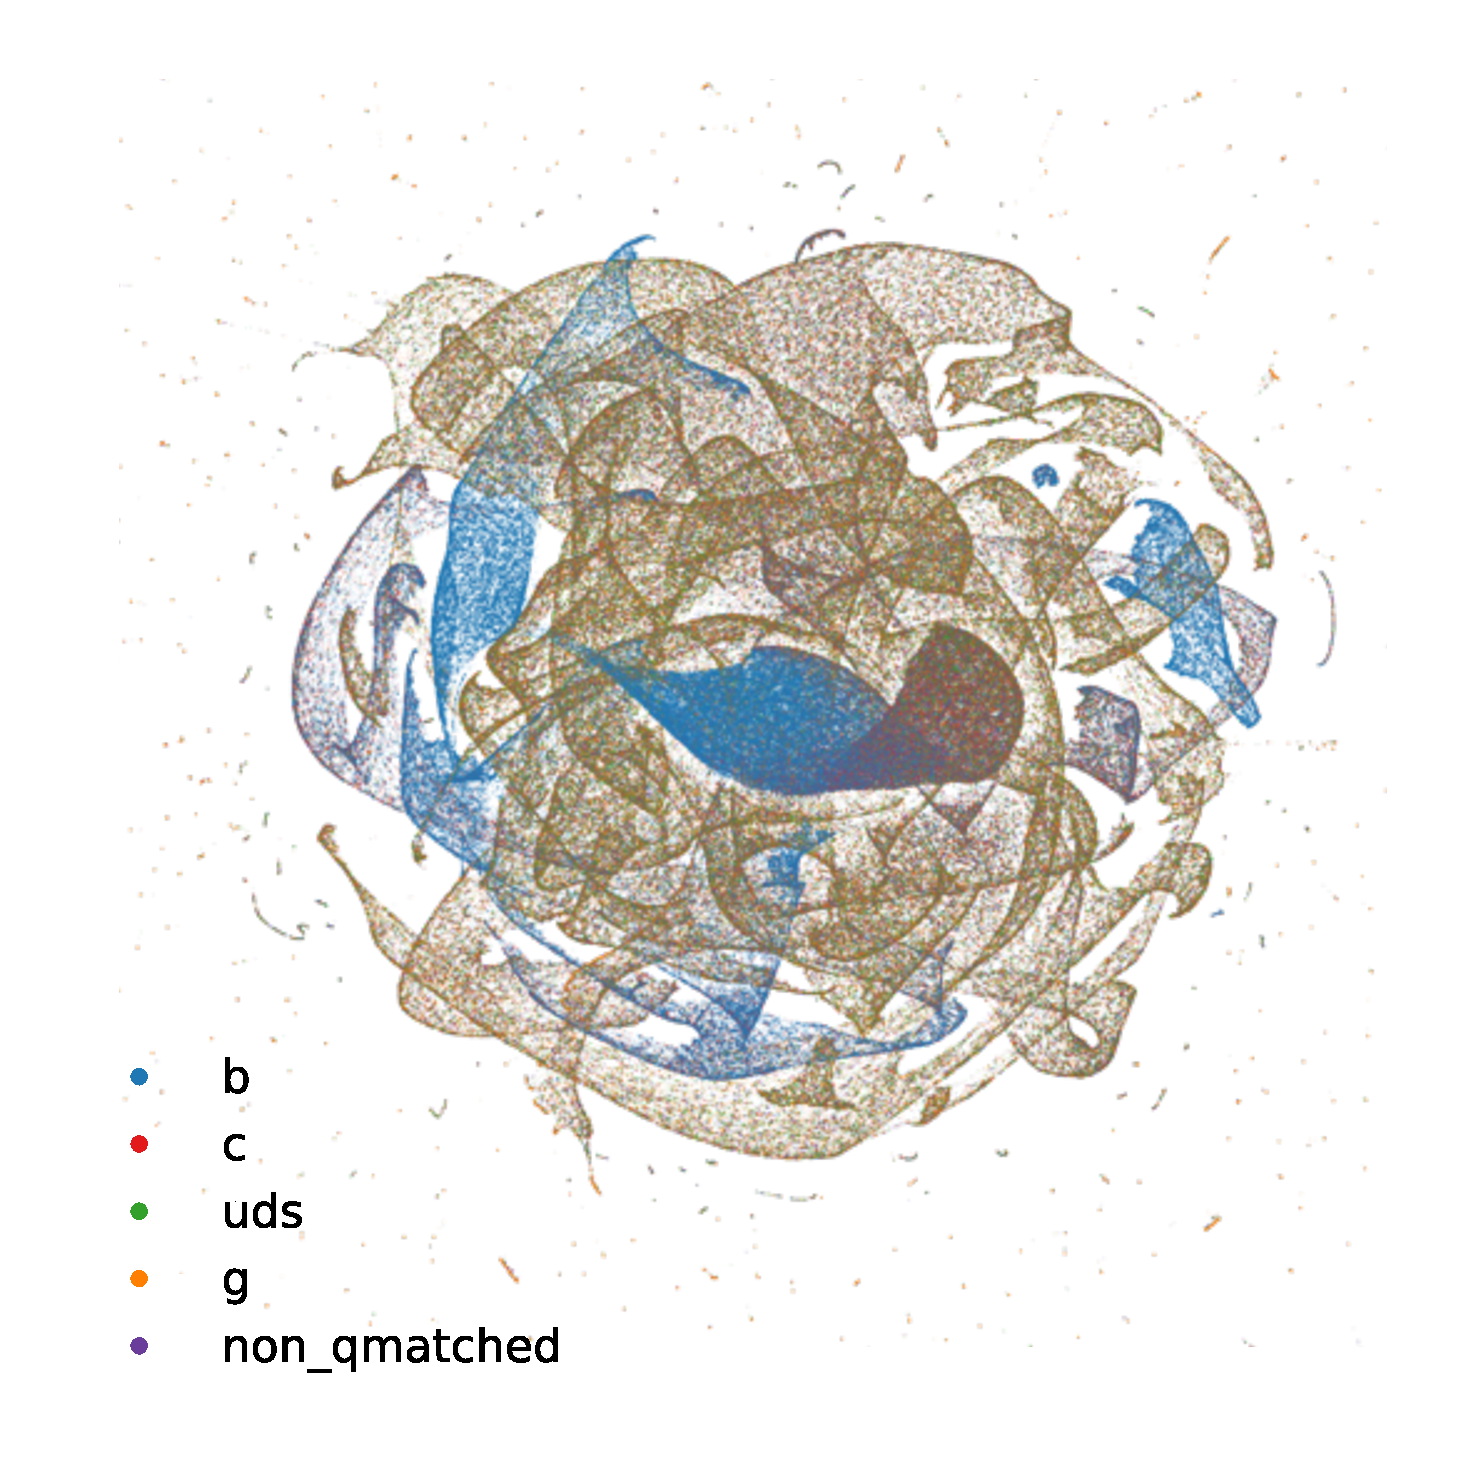
\includegraphics[draft=true, width=0.95\textwidth, trim=50 45 50 50, clip]{figures/quarks/df_UMAP-X=1078089-n_neighbors=250-min_dist=0.2-metric=euclidean-input2b_njet=3_algorithm=UMAP_single.pdf}
  \caption[UMAP visualization of vertex variables for 3-jet events]
          {UMAP visualization of vertex variables for 3-jet events.} 
  \label{fig:q:UMAP_vertex_3j}
\end{marginfigure}

\begin{marginfigure}
  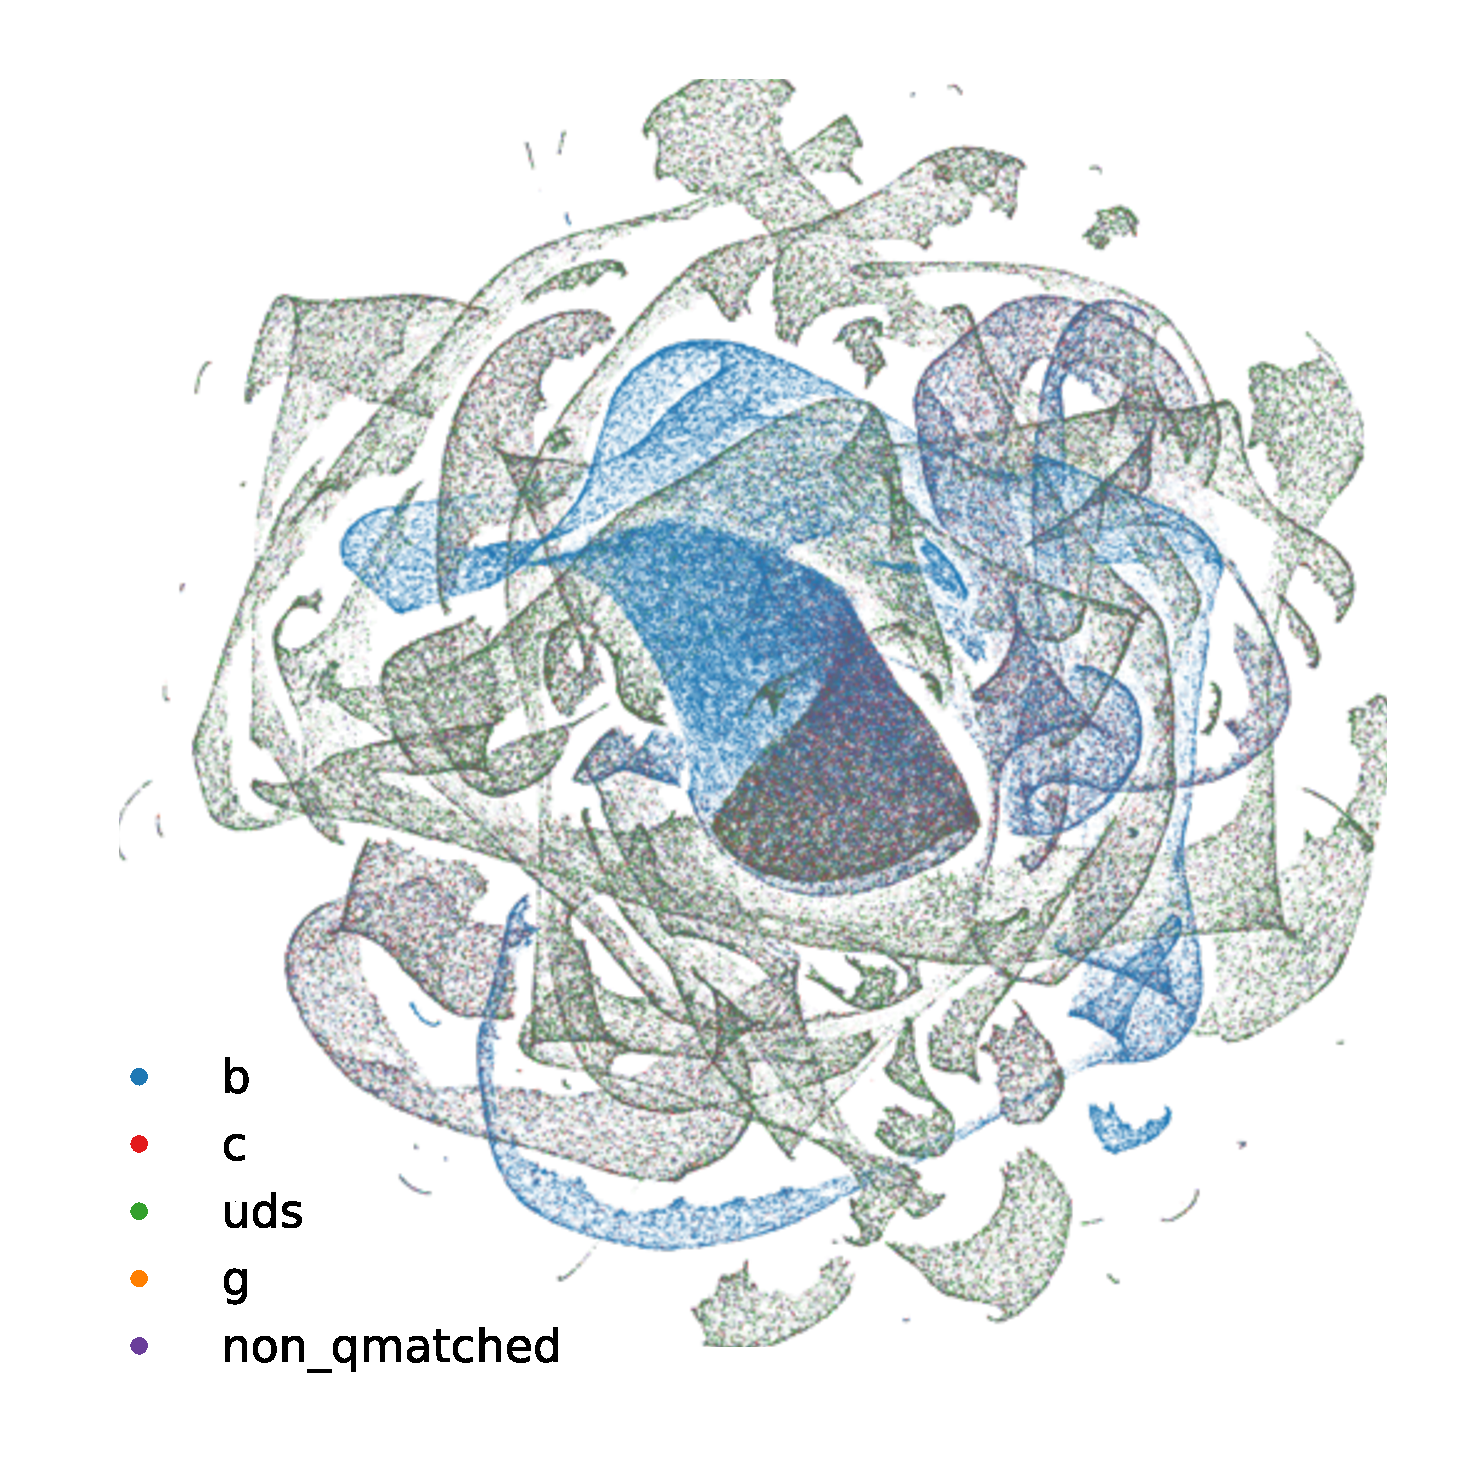
\includegraphics[draft=true, width=0.95\textwidth, trim=50 45 50 50, clip]{figures/quarks/df_UMAP-X=729358-n_neighbors=250-min_dist=0.2-metric=euclidean-input2b_njet=2_algorithm=UMAP_single.pdf}
  \caption[UMAP visualization of vertex variables for 2-jet events]
          {UMAP visualization of vertex variables for 2-jet events.} 
  \label{fig:q:UMAP_vertex_2j}
\end{marginfigure}

The UMAP algorithm has several hyperparameters, where two of the most important ones are the number of neighbors \code{n_neighbors} which controls the priority between correctly preserving the global versus the local structure, and the \code{min_dist} which defines how tightly together UMAP is allowed to cluster the points in the low-dimensional representation. To properly choose the best combination of \code{n_neighbors} and \code{min_dist} a grid search with \code{n_neighbors}~$\in \{10, 50, 100, 250 \}$ and \code{min_dist}~$\in \{0, 0.2, 0.5\}$ is performed. This is shown for 4-jet events in Figure~\ref{fig:q:UMAP_vertex_all} in the appendix. In this case the choice of best combination of \code{n_neighbors} and \code{min_dist} is subjective at best, but it was judged by the author that \code{n_neighbors}~$=250$ and \code{min_dist}~$0.2$ gave the best compromise between preserving local and global structure. The results of running UMAP on 4-jet events can be seen in Figure~\ref{fig:q:UMAP_vertex_2j}. Here the millions of points are plotted using Datashader \autocite{bednarDatashaderRevealingStructure2019} to avoid overplotting and colored according to the jet type. From the figure it is seen how there are some clear, blue $b$-jet clusters, however, most of the data seem to be a mix of $g$- and $uds$-jets. The plots with the same UMAP parameters for 3-jet and 2-jet events are seen in Figure~\ref{fig:q:UMAP_vertex_3j} and \ref{fig:q:UMAP_vertex_2j}. 

These figures suggests that it should be possible to discriminate the $b$-jets from the other jets somewhat, however, no clear separation is expected. The t-SNE algorithm was also tested but showed inferior performance compared to UMAP, see Figure~\ref{fig:q:tsne_vertex} in the appendix for an example of this.



The correlation between the vertex variables can be seen in Figure~\ref{fig:q:correlation_vertex_all}, where the upper diagonal shows the linear correlation $\rho$ and the lower diagonal shows the (estimate of the) MIC non-linear correlation $\mathrm{MIC}_e$. Here it ca be seen that \code{projet} and \code{bqvjet} correlate mostly whereas the other variables correlate a lot less. Had they all correlated a lot, it would be more difficult to extract any meaningful insights from the system at it would contain less information. 

\begin{figure}%
  \centering
  \subfloat[2-jet events]{{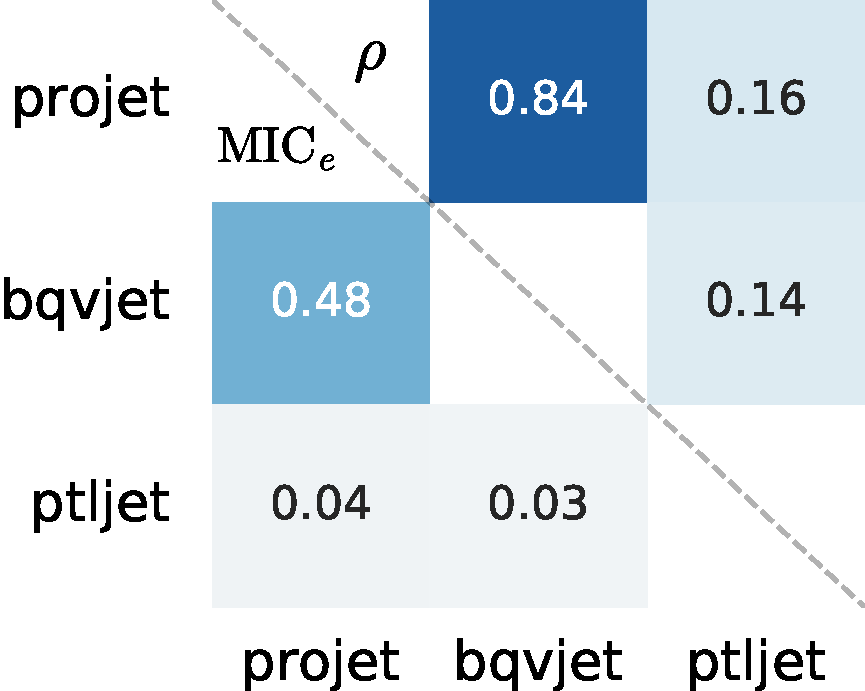
\includegraphics[width=0.31\textwidth]{figures/quarks/correlations_vertex_vars-down_sample=1.00-ML_vars=vertex-selection=b-ejet_min=4-n_iter_RS_lgb=99-n_iter_RS_xgb=9-cdot_cut=0.90-version=19_njet=2.pdf}}}%
  \;
  \subfloat[3-jet events]{{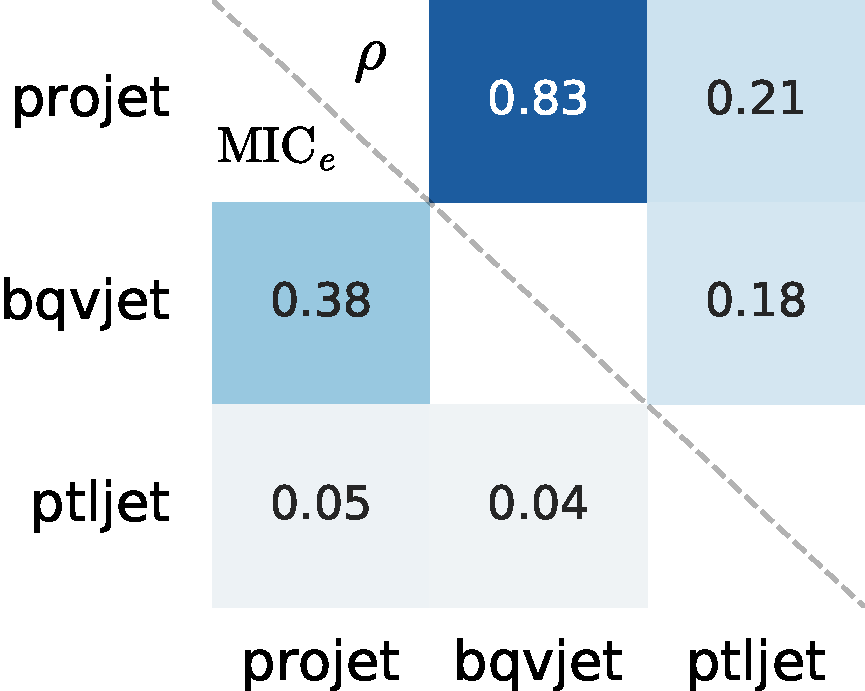
\includegraphics[width=0.31\textwidth]{figures/quarks/correlations_vertex_vars-down_sample=1.00-ML_vars=vertex-selection=b-ejet_min=4-n_iter_RS_lgb=99-n_iter_RS_xgb=9-cdot_cut=0.90-version=19_njet=3.pdf} }}%
  \subfloat[4-jet events]{{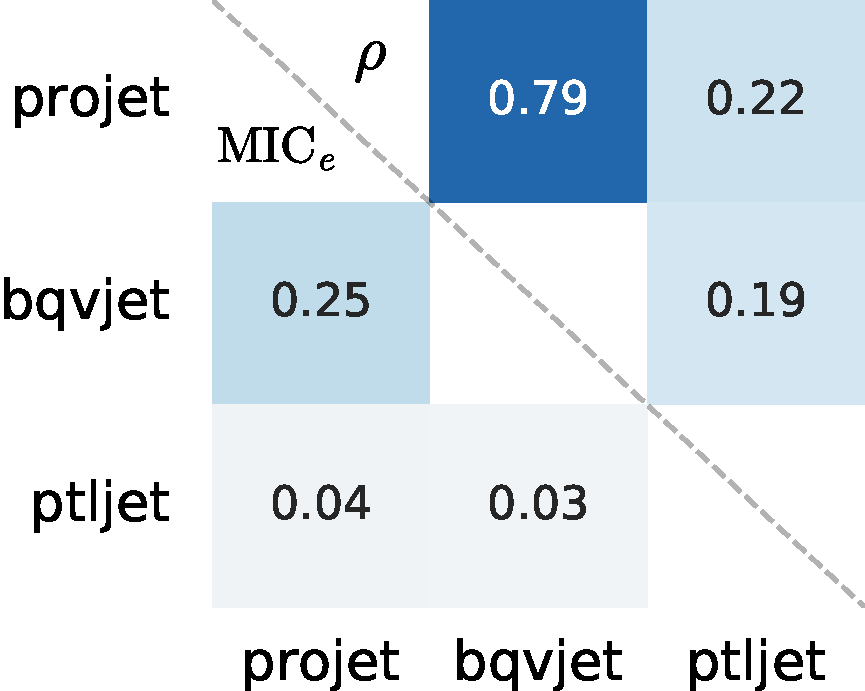
\includegraphics[width=0.31\textwidth]{figures/quarks/correlations_vertex_vars-down_sample=1.00-ML_vars=vertex-selection=b-ejet_min=4-n_iter_RS_lgb=99-n_iter_RS_xgb=9-cdot_cut=0.90-version=19_njet=4.pdf} }}%
  \caption[Correlation of Vertex Variables]{Correlation of the three vertex variables for 2-, 3- and 4-jet events.}%
  \label{fig:q:correlation_vertex_all}%
\end{figure}
\vspace{0.5cm}

% \begin{figure}
%   \centering
%   % \vspace*{-\abovecaptionskip}
%   \subfloat[\label{fig:q:correlation_vertex_2j}]{\;}
%   \subfloat[\label{fig:q:correlation_vertex_2j}]{\;}
%   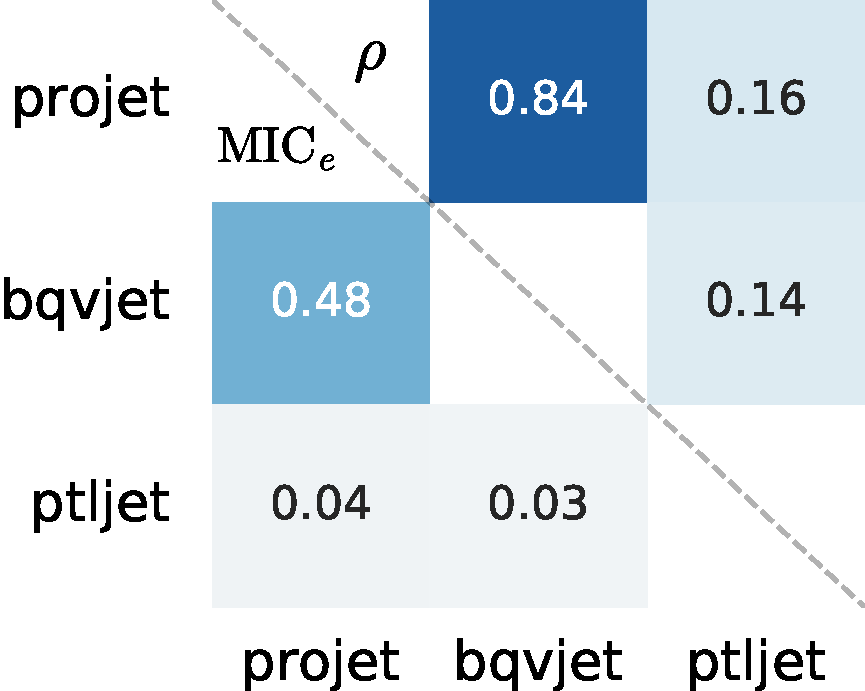
\includegraphics[width=0.28\textwidth]{figures/quarks/correlations_vertex_vars-down_sample=1.00-ML_vars=vertex-selection=b-ejet_min=4-n_iter_RS_lgb=99-n_iter_RS_xgb=9-cdot_cut=0.90-version=19_njet=2.pdf}\hfil
%   \subfloat[\label{fig:q:correlation_vertex_3j}]{\;}
%   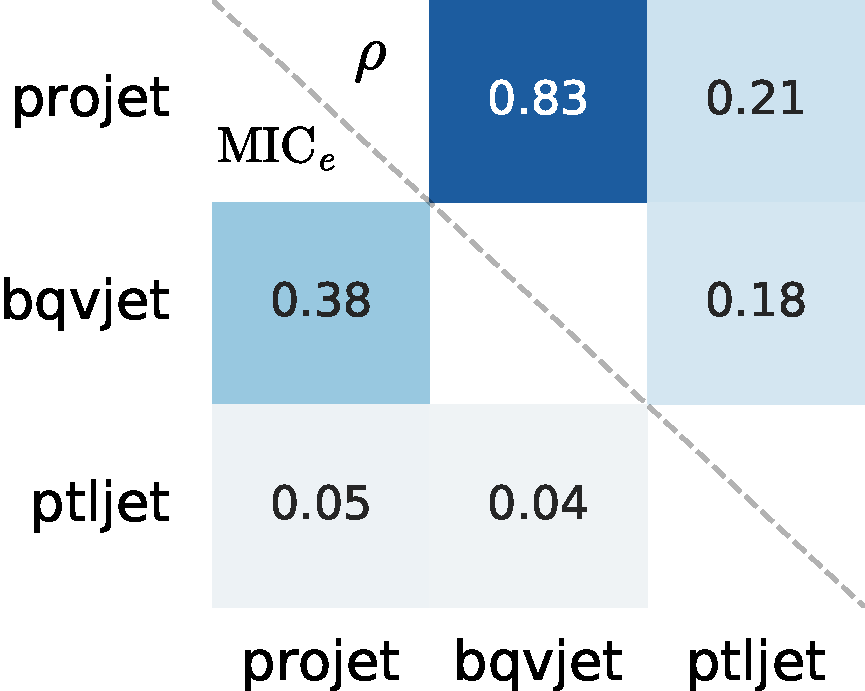
\includegraphics[width=0.28\textwidth]{figures/quarks/correlations_vertex_vars-down_sample=1.00-ML_vars=vertex-selection=b-ejet_min=4-n_iter_RS_lgb=99-n_iter_RS_xgb=9-cdot_cut=0.90-version=19_njet=3.pdf}\hfil
%   \subfloat[\label{fig:q:correlation_vertex_4j}]{\;}
%   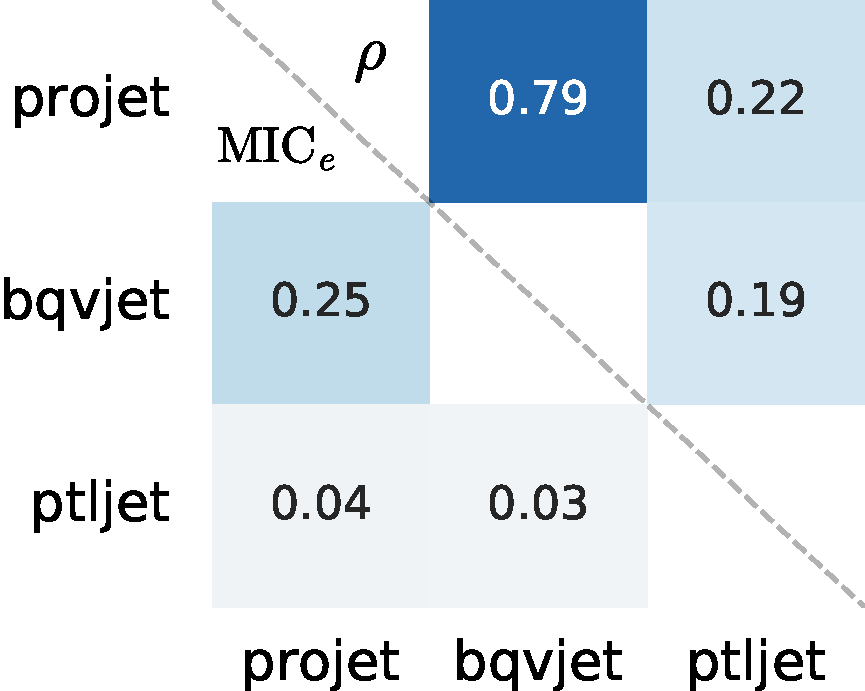
\includegraphics[width=0.28\textwidth]{figures/quarks/correlations_vertex_vars-down_sample=1.00-ML_vars=vertex-selection=b-ejet_min=4-n_iter_RS_lgb=99-n_iter_RS_xgb=9-cdot_cut=0.90-version=19_njet=4.pdf}\hfil
%   \caption[Correlation of Vertex Variables]{Correlation of the three vertex variables for . 
%            Subplot ~\protect\subref{fig:q:correlation_vertex_2j} shows the date of the sale, 
%            Subplot ~\protect\subref{fig:q:correlation_vertex_3j} shows the type of residence,
%            Subplot ~\protect\subref{fig:q:correlation_vertex_4j} shows the area og the house.}
%   \label{fig:q:correlation_vertex_all}
%   \vspace{\abovecaptionskip}
% \end{figure}


\FloatBarrier
\section{Loss and Evaluation Function}
\label{sec:q:loss_evaluation_function}

In contrary to the housing prices subproject the goal is to predict the class of particles. The combination of this being a \emph{classification} problem (compared to a regression problem) along with the fact all the variables are actual measurements from a particle physics accelerator means that the issue of outliers is negligible. This also means that the problem of finding a robust loss function is non-existent since the in classification loss is already bounded in the $[0, 1]$-interval. 


\FloatBarrier
\section[b-Tagging Analysis]{$b$-Tagging Analysis}
\label{sec:q:b_tagging_analysis}

The ability to discriminate between the different types of particles produced in a collision is obviously import to understand the results. Today much work go into tagging algorithms from $b$-tagging in ATLAS and CMS \autocite{scodellaroTaggingATLASCMS2017} but this work started even decades ago. That $b$-quarks are tagged specifically is both due to $b$-quarks having more unique characteristics compared to e.g. $c$-quarks and are thus easier to tag, but also the fact that $b$-quarks are the second-heaviest of the quarks and are measured to better understand CP\sidenote{Short for charge-parity.}-violation at LHC-b, contributes to the choice of tagging $b$-quarks. In ALEPH \citet{proriolTAGGINGQUARKEVENTS1991} started the work of comparing different methods for $b$-tagging already in \num{1991}. They concluded that a neural network had the best performance compared to e.g. a linear (Fisher) discriminant. The neural network used was a 3-layer neural network (NN) trained on nine variables and the output \code{nnbjet}. For this of this project this pre-trained network will be called NNB. 

The data are split\sidenote{After removing all low-energy jets such that all events that contain any jets with an energy of less than \SI{4}{\GeV} are removed.} into training and test sets in such a way that the individual jets in an event are not split. As such, the splitting is performed at event-scale in a $(80:20)\si{\percent}$ train-test ratio. 

\newpage
\begin{figure}
  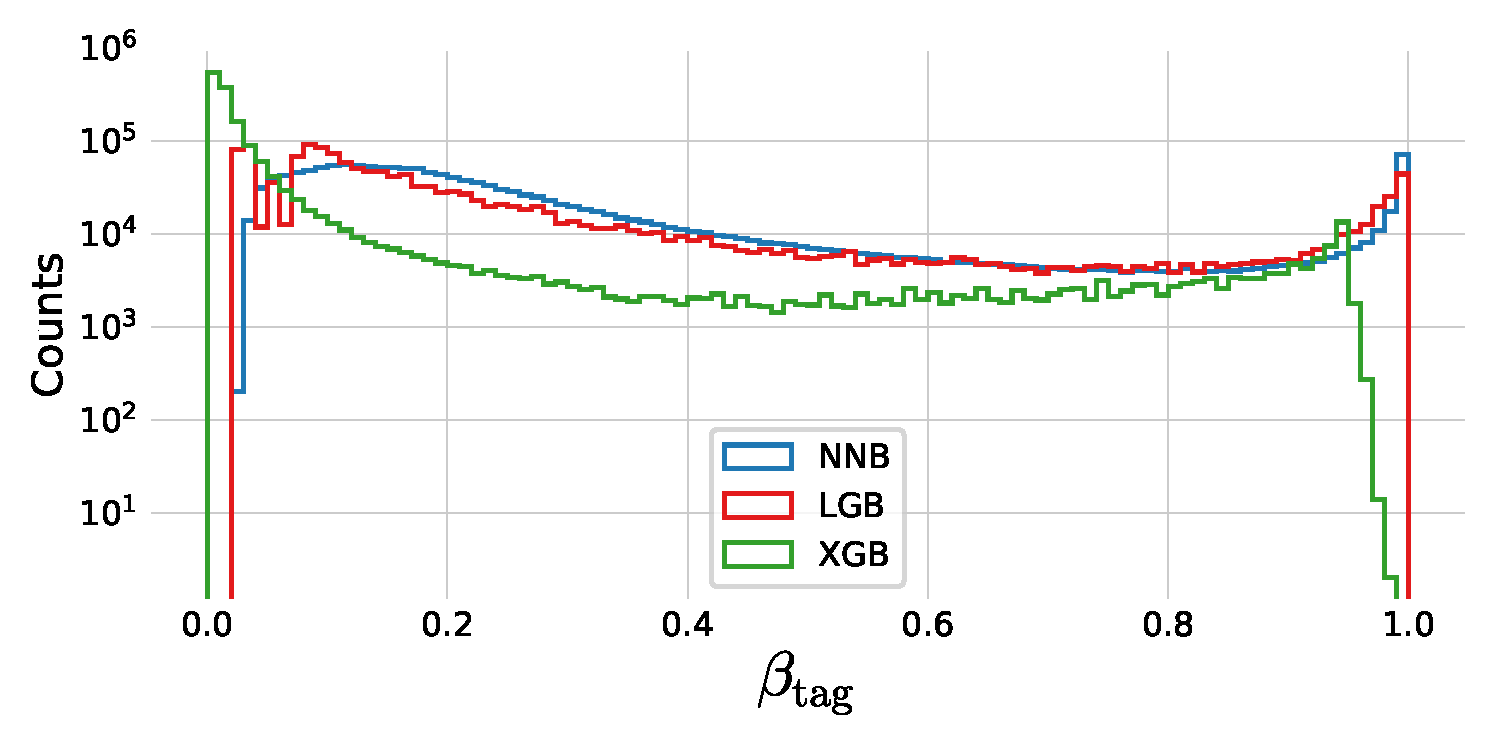
\includegraphics[width=0.95\textwidth, trim=0 0 0 30, clip]{figures/quarks/y_pred_3_jet_hist-down_sample=1.00-ML_vars=vertex-selection=b-ejet_min=4-n_iter_RS_lgb=99-n_iter_RS_xgb=9-cdot_cut=0.90-version=19.pdf}
  \caption[b-tag scores in 3-jet events]
          {Histogram of b-tag scores (model prediction) in 3-jet events for \textcolor{blue}{NNB} (the neural network trained by ATLAS, also called \code{nnbjet}) in blue, \textcolor{red}{XGB} in red, and \textcolor{green}{XGB} in green. We see that the XGB predictions closely match those of NNB which is a good confirmation of a successful fit.  
          } 
  \label{fig:q:btag_scores_3j}
\end{figure}




\begin{figure}
  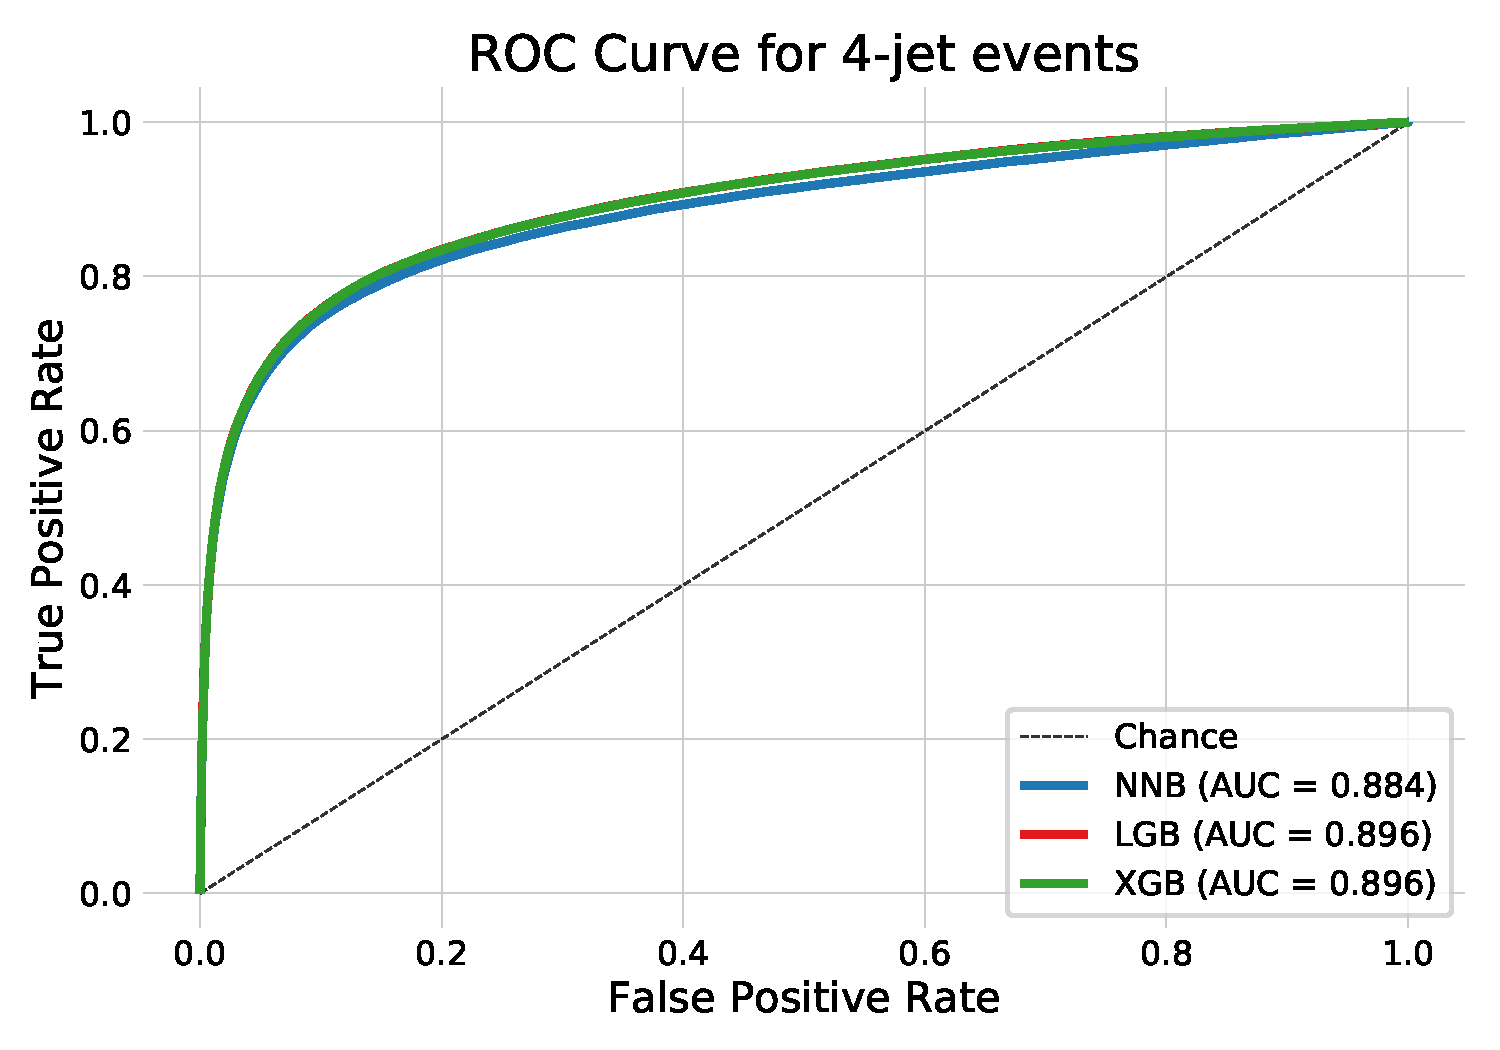
\includegraphics[width=0.95\textwidth, trim=10 10 10 40, clip]{figures/quarks/ROC_4_jet-down_sample=1.00-ML_vars=vertex-selection=b-ejet_min=4-n_iter_RS_lgb=99-n_iter_RS_xgb=9-cdot_cut=0.90-version=19.pdf}
  \caption[ROC curve for b-tag in 4-jet events]
          {ROC curve of the three b-tag models in 3-jet events for \textcolor{blue}{NNB} (the neural network trained by ATLAS, also called \code{nnbjet}) in blue, \textcolor{red}{XGB} in red, and \textcolor{green}{XGB} in green. In the legend the Area Under Curve (AUC) is also shown. Notice that the XGB and XGB models share performance and it is thus due to overplotting that only the green line for XGB can be seen. In the particle physics community False Positive Rate (FPR) is sometimes better known as background efficiency and True Positive Rate (TPR) as signal efficiency.  
          } 
  \label{fig:q:roc_btag_4j}
\end{figure}




\begin{figure}
  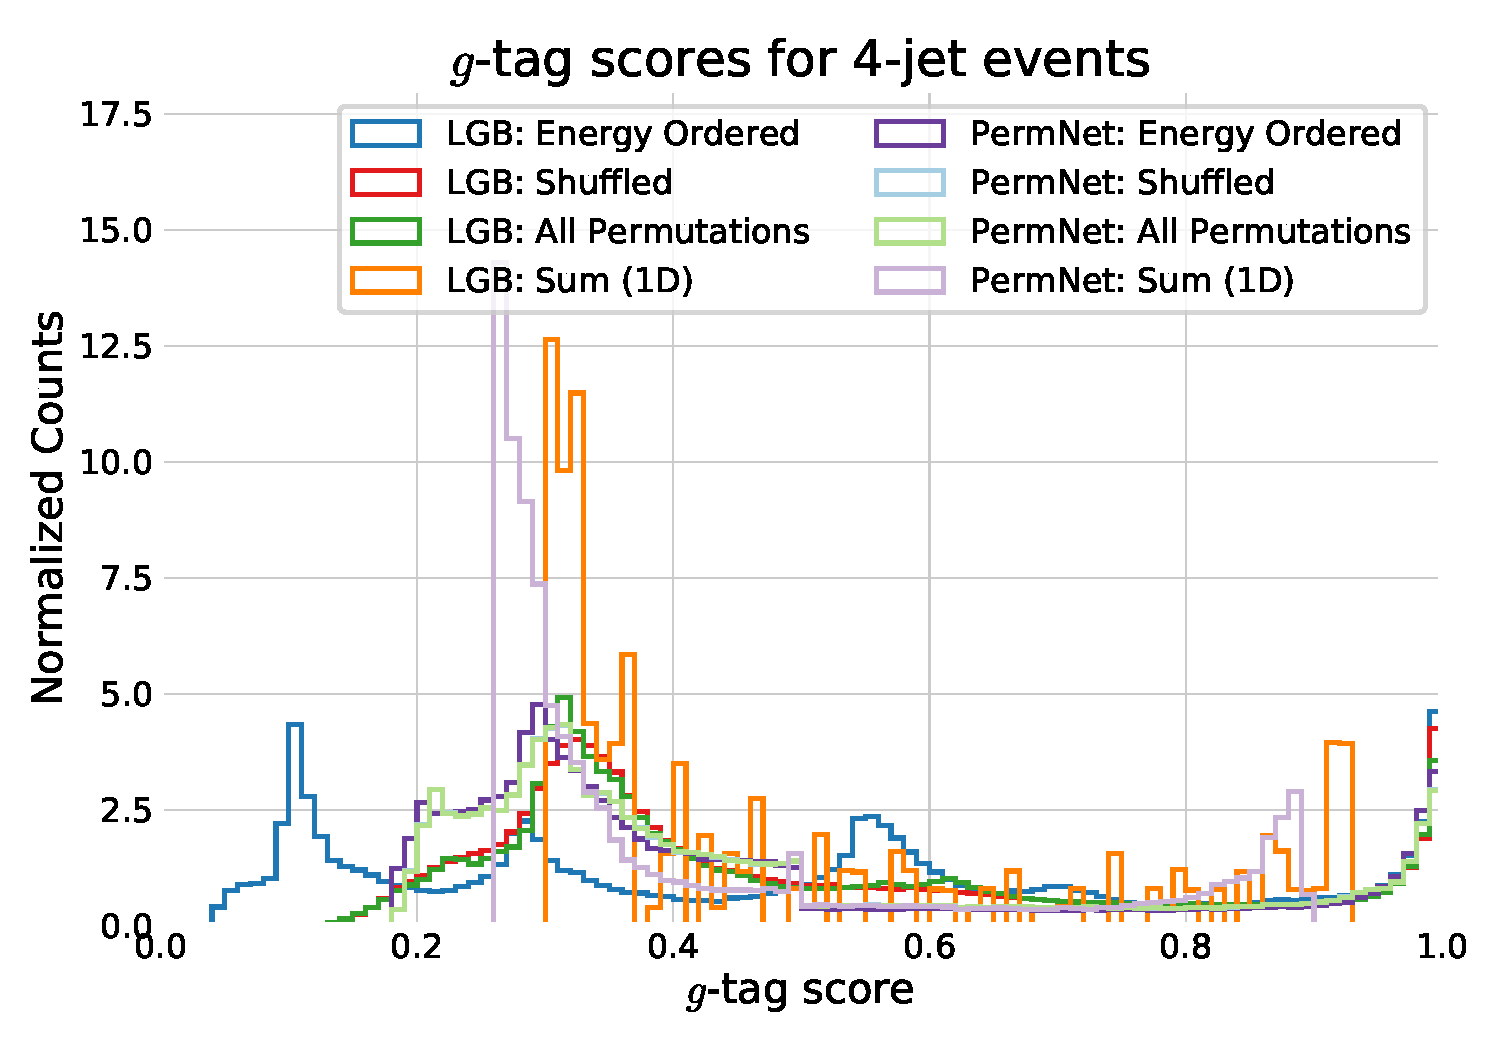
\includegraphics[width=0.95\textwidth, trim=10 10 10 40, clip]{figures/quarks/gtag_y_pred_4_jet_hist-down_sample=1.00-ML_vars=vertex-selection=b-ejet_min=4-n_iter_RS_lgb=99-n_iter_RS_xgb=9-cdot_cut=0.90-version=19.pdf}
  \caption[g-tag scores in 4-jet events]
          {
            Histogram of g-tag scores (model prediction) in 4-jet events for \textcolor{blue}{XGB: Energy Ordered} in blue, \textcolor{red}{XGB: Shuffled} in red, \textcolor{green}{XGB: All Permutations} in green, \textcolor{orange}{XGB: Sum 1D} in orange, \textcolor{purple}{PermNet: Energy Ordered} in purple, \textcolor{light-blue}{PermNet: Shuffled} in light-blue, \textcolor{light-green}{PermNet: All Permutations} in light-green, \textcolor{light-purple}{PermNet: Sum 1D} in light-purple.  Here XGB and PermNet are the two different type of models and \q{Energy Ordered}, \q{Shuffled}, \q{All Permutations}, and \q{Sum 1D} are the different methods used for making the input data permutation invariant.  
          }   
  \label{fig:q:gtag_scores_4j}
\end{figure}


\begin{figure}
  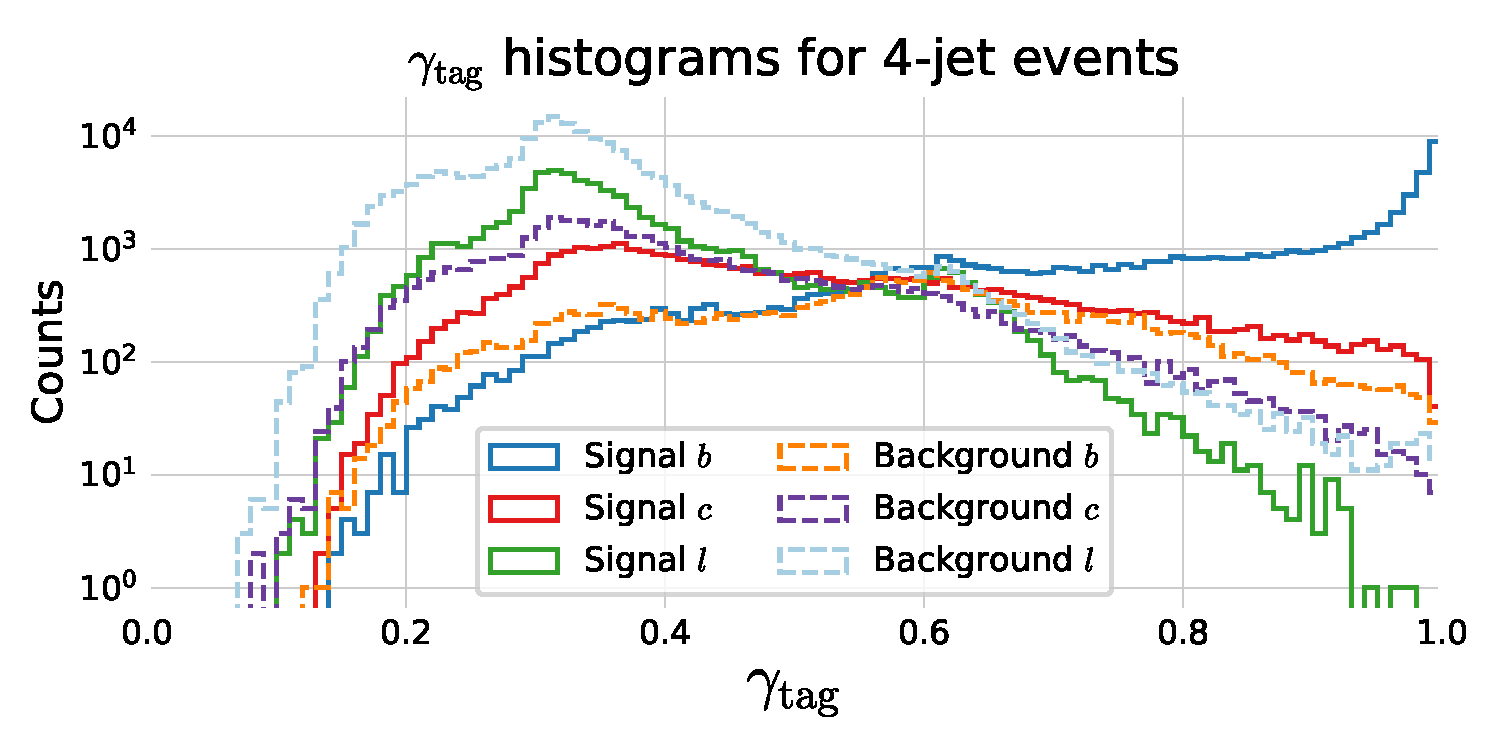
\includegraphics[width=0.95\textwidth, trim=10 10 10 40, clip]{figures/quarks/gtag-histogram-sigbkg-down_sample=1.00-ML_vars=vertex-selection=b-ejet_min=4-n_iter_RS_lgb=99-n_iter_RS_xgb=9-cdot_cut=0.90-version=19-njet=4.pdf}
  \caption[g-tag scores in 4-jet events for signal and background]
          {Histogram of g-tag scores (model prediction) from the XGB-model in 4-jet events for \textcolor{blue}{b signal} in blue, \textcolor{red}{c signal} in red, \textcolor{green}{l signal} in green, \textcolor{orange}{b background} in orange, \textcolor{purple}{c background} in purple, \textcolor{light-blue}{l background} in light-blue.
          } 
  \label{fig:q:gtag_scores_4j_sig_bkg}
\end{figure}





\begin{figure}
  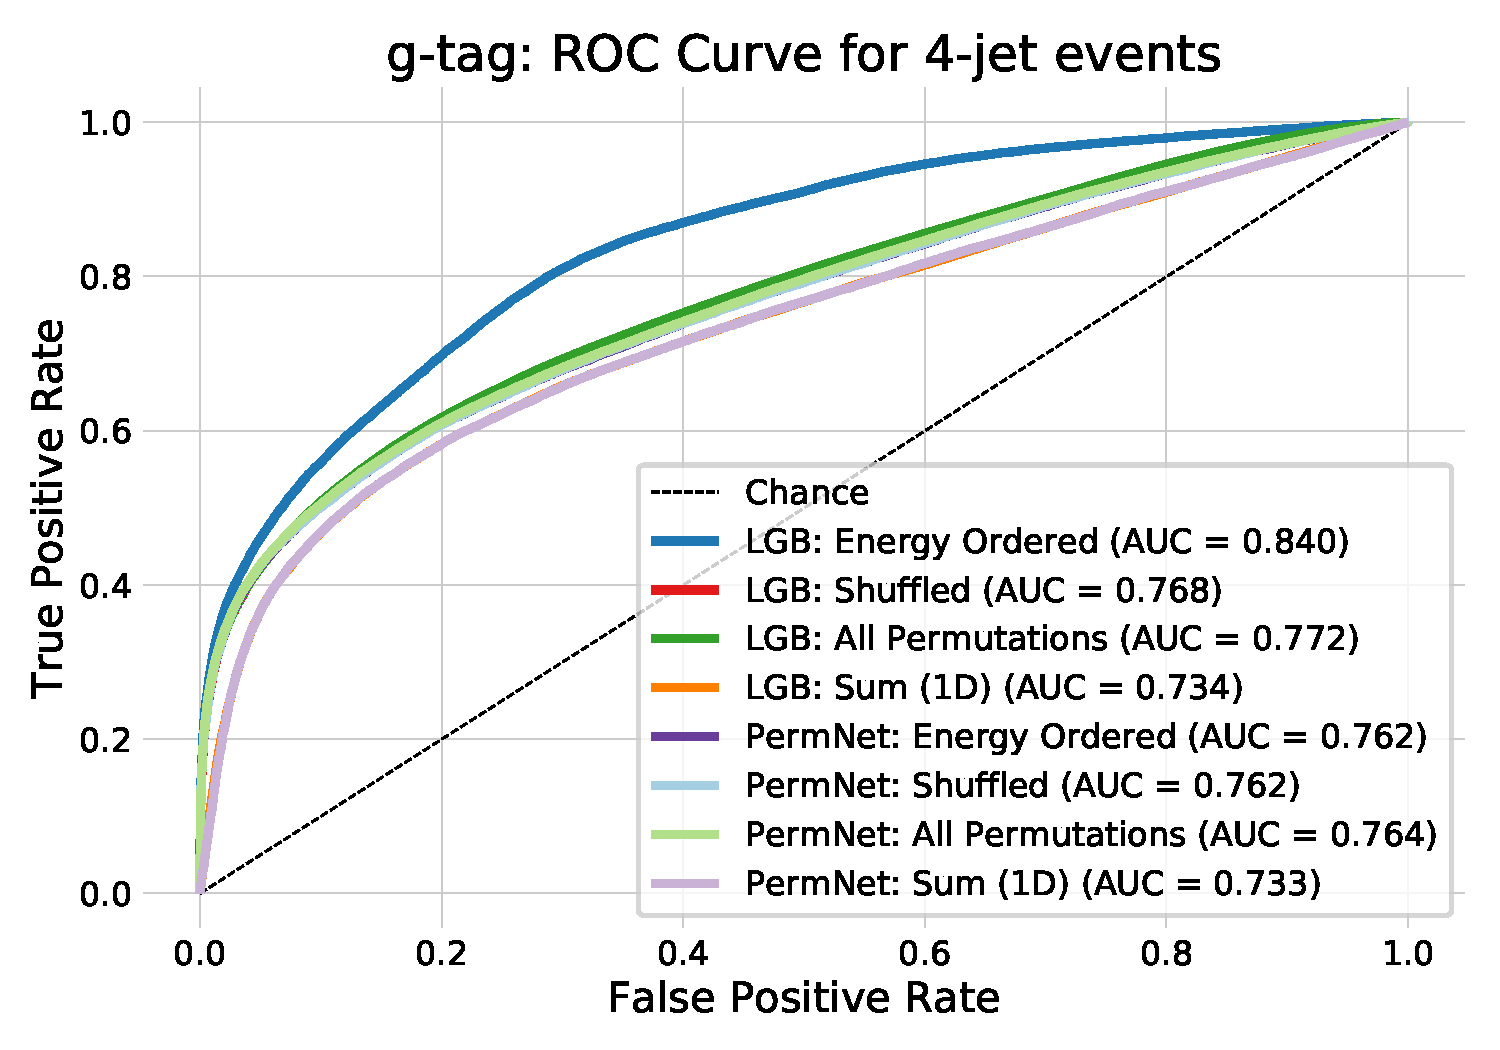
\includegraphics[width=0.95\textwidth, trim=10 10 10 40, clip]{figures/quarks/gtag_ROC_4_jet-down_sample=1.00-ML_vars=vertex-selection=b-ejet_min=4-n_iter_RS_lgb=99-n_iter_RS_xgb=9-cdot_cut=0.90-version=19.pdf}
  \caption[ROC curve for g-tag in 4-jet events]
          {ROC curve of the eight g-tag models in 4-jet events. First one in dashed black is the ROC curve that you get by random chance. The colors are the same as in \figref{fig:q:gtag_scores_4j} and in the legend also the Area Under the ROC curve (AUC) is shown. 
          Notice that the XGB model which uses the energy ordered data produced the best model, however, this model is not permutation invariant. Of the permutation invariant models (the rest), the XGB model trained on all permutations of the b-tags performs highest. The lowest performing models are the two models trained only on the 1-dimensional sum of b-tags, as expected, however, still with a better performance than expected by the author.  
          } 
  \label{fig:q:roc_gtag_4j}
\end{figure}





\begin{figure}
  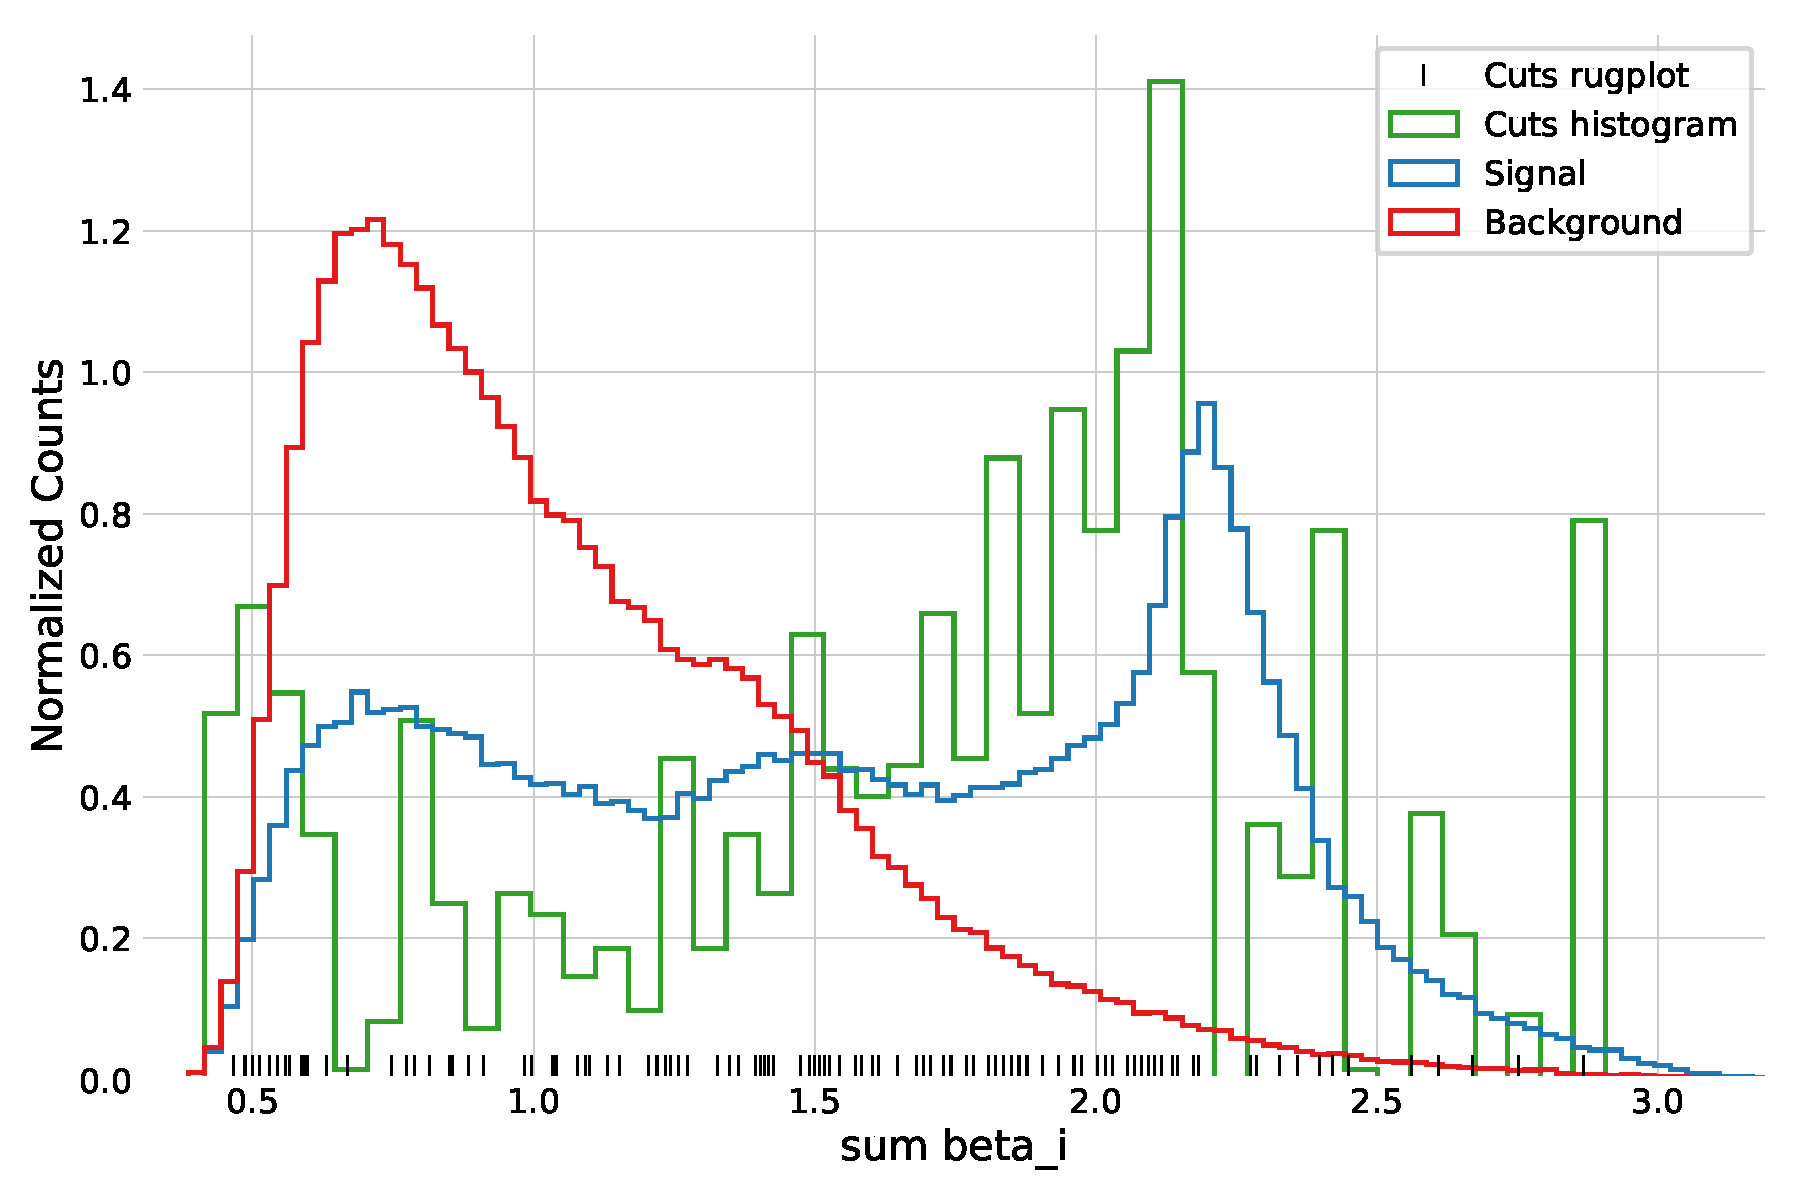
\includegraphics[width=0.95\textwidth, trim=10 10 10 20, clip]{figures/quarks/gtag_sum_method_njet=4-down_sample=1.00-ML_vars=vertex-selection=b-ejet_min=4-n_iter_RS_lgb=99-n_iter_RS_xgb=9-cdot_cut=0.90-version=19.pdf}
  \caption[1D Sum Model Cuts for 4-jets]
          {Histogram of the distribution of \textcolor{blue}{signal} in blue and \textcolor{red}{background} in red for 1-dimensional sum of b-tags training data. A histogram of the \textcolor{green}{cut values} from the XGB model trained on this data is shown in green together with a rug plot of the cut values in black. Notice how most of the cuts match up with the signal peak at around a $\sum \beta_i \sim 2.1$, however, there are also quite a lot of cuts around $\sum \beta_i \sim 0.5$.
          } 
  \label{fig:q:1d_sum_model_cuts_4j}
\end{figure}


\begin{figure}
  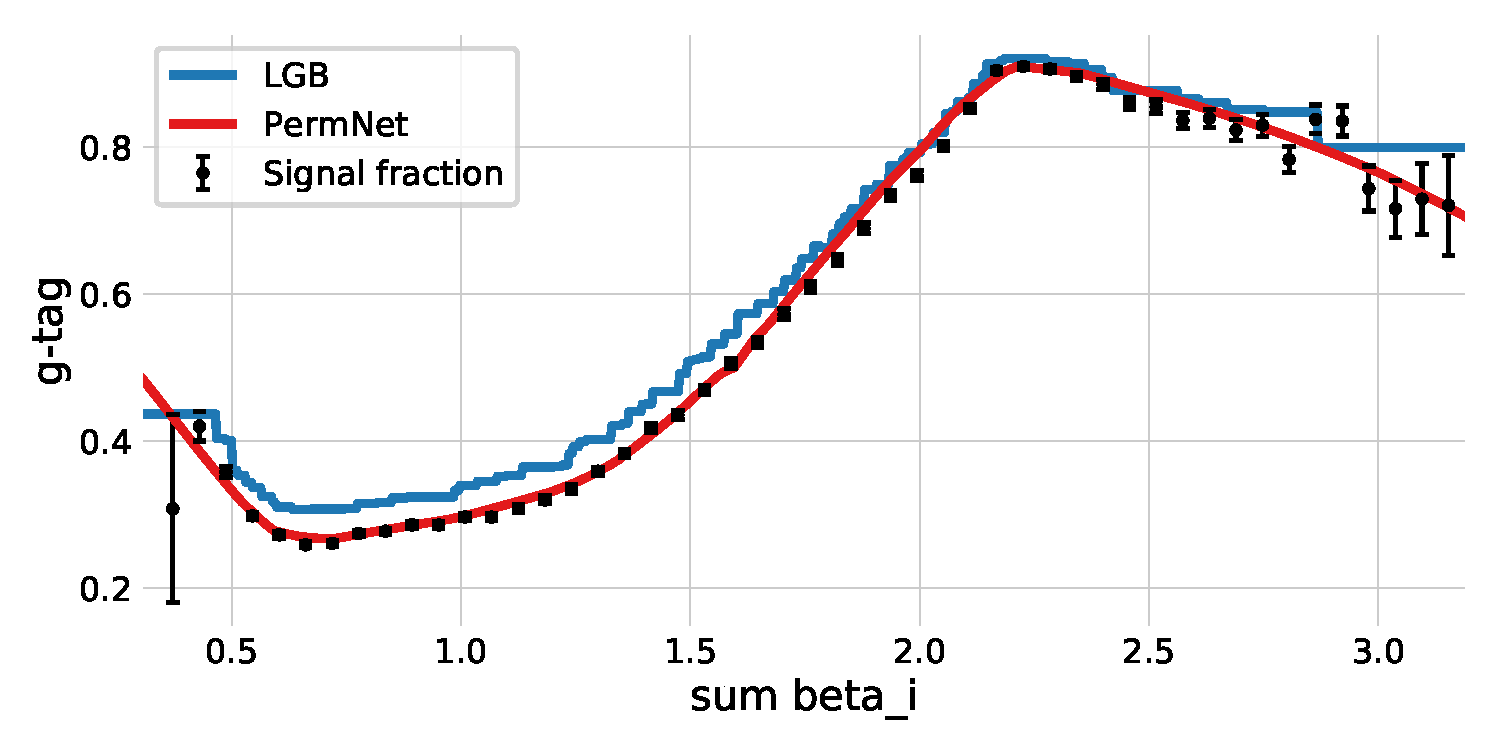
\includegraphics[width=0.95\textwidth, trim=10 10 10 20, clip]{figures/quarks/gtag_sum_models_njet=4-down_sample=1.00-ML_vars=vertex-selection=b-ejet_min=4-n_iter_RS_lgb=99-n_iter_RS_xgb=9-cdot_cut=0.90-version=19.pdf}
  \caption[1D Sum Models Predictions and Signal Fraction for 4-jets]
          {Plot of the (1D) g-tag scores as a function of $\sum \beta_i$ for the \textcolor{blue}{XGB} model in blue and the \textcolor{red}{PermNet} model in red. Here the g-tag scores are just the models' output values when input a uniformly spaced grid of $\sum \beta_i$ values between 0 and 4. The signal fraction (based on the signal and background histograms in \figref{fig:q:1d_sum_model_cuts_4j}) is plotted as black error bars where the size of the error bars is based on the propagated uncertainties of the signal and background histogram assuming Poissonian statistics. Notice how both models capture the overall trend of the signal fraction with the PermNet being particularly close. 
          } 
  \label{fig:q:1d_sum_models_signal_fraction_4j}
\end{figure}




\begin{figure}
  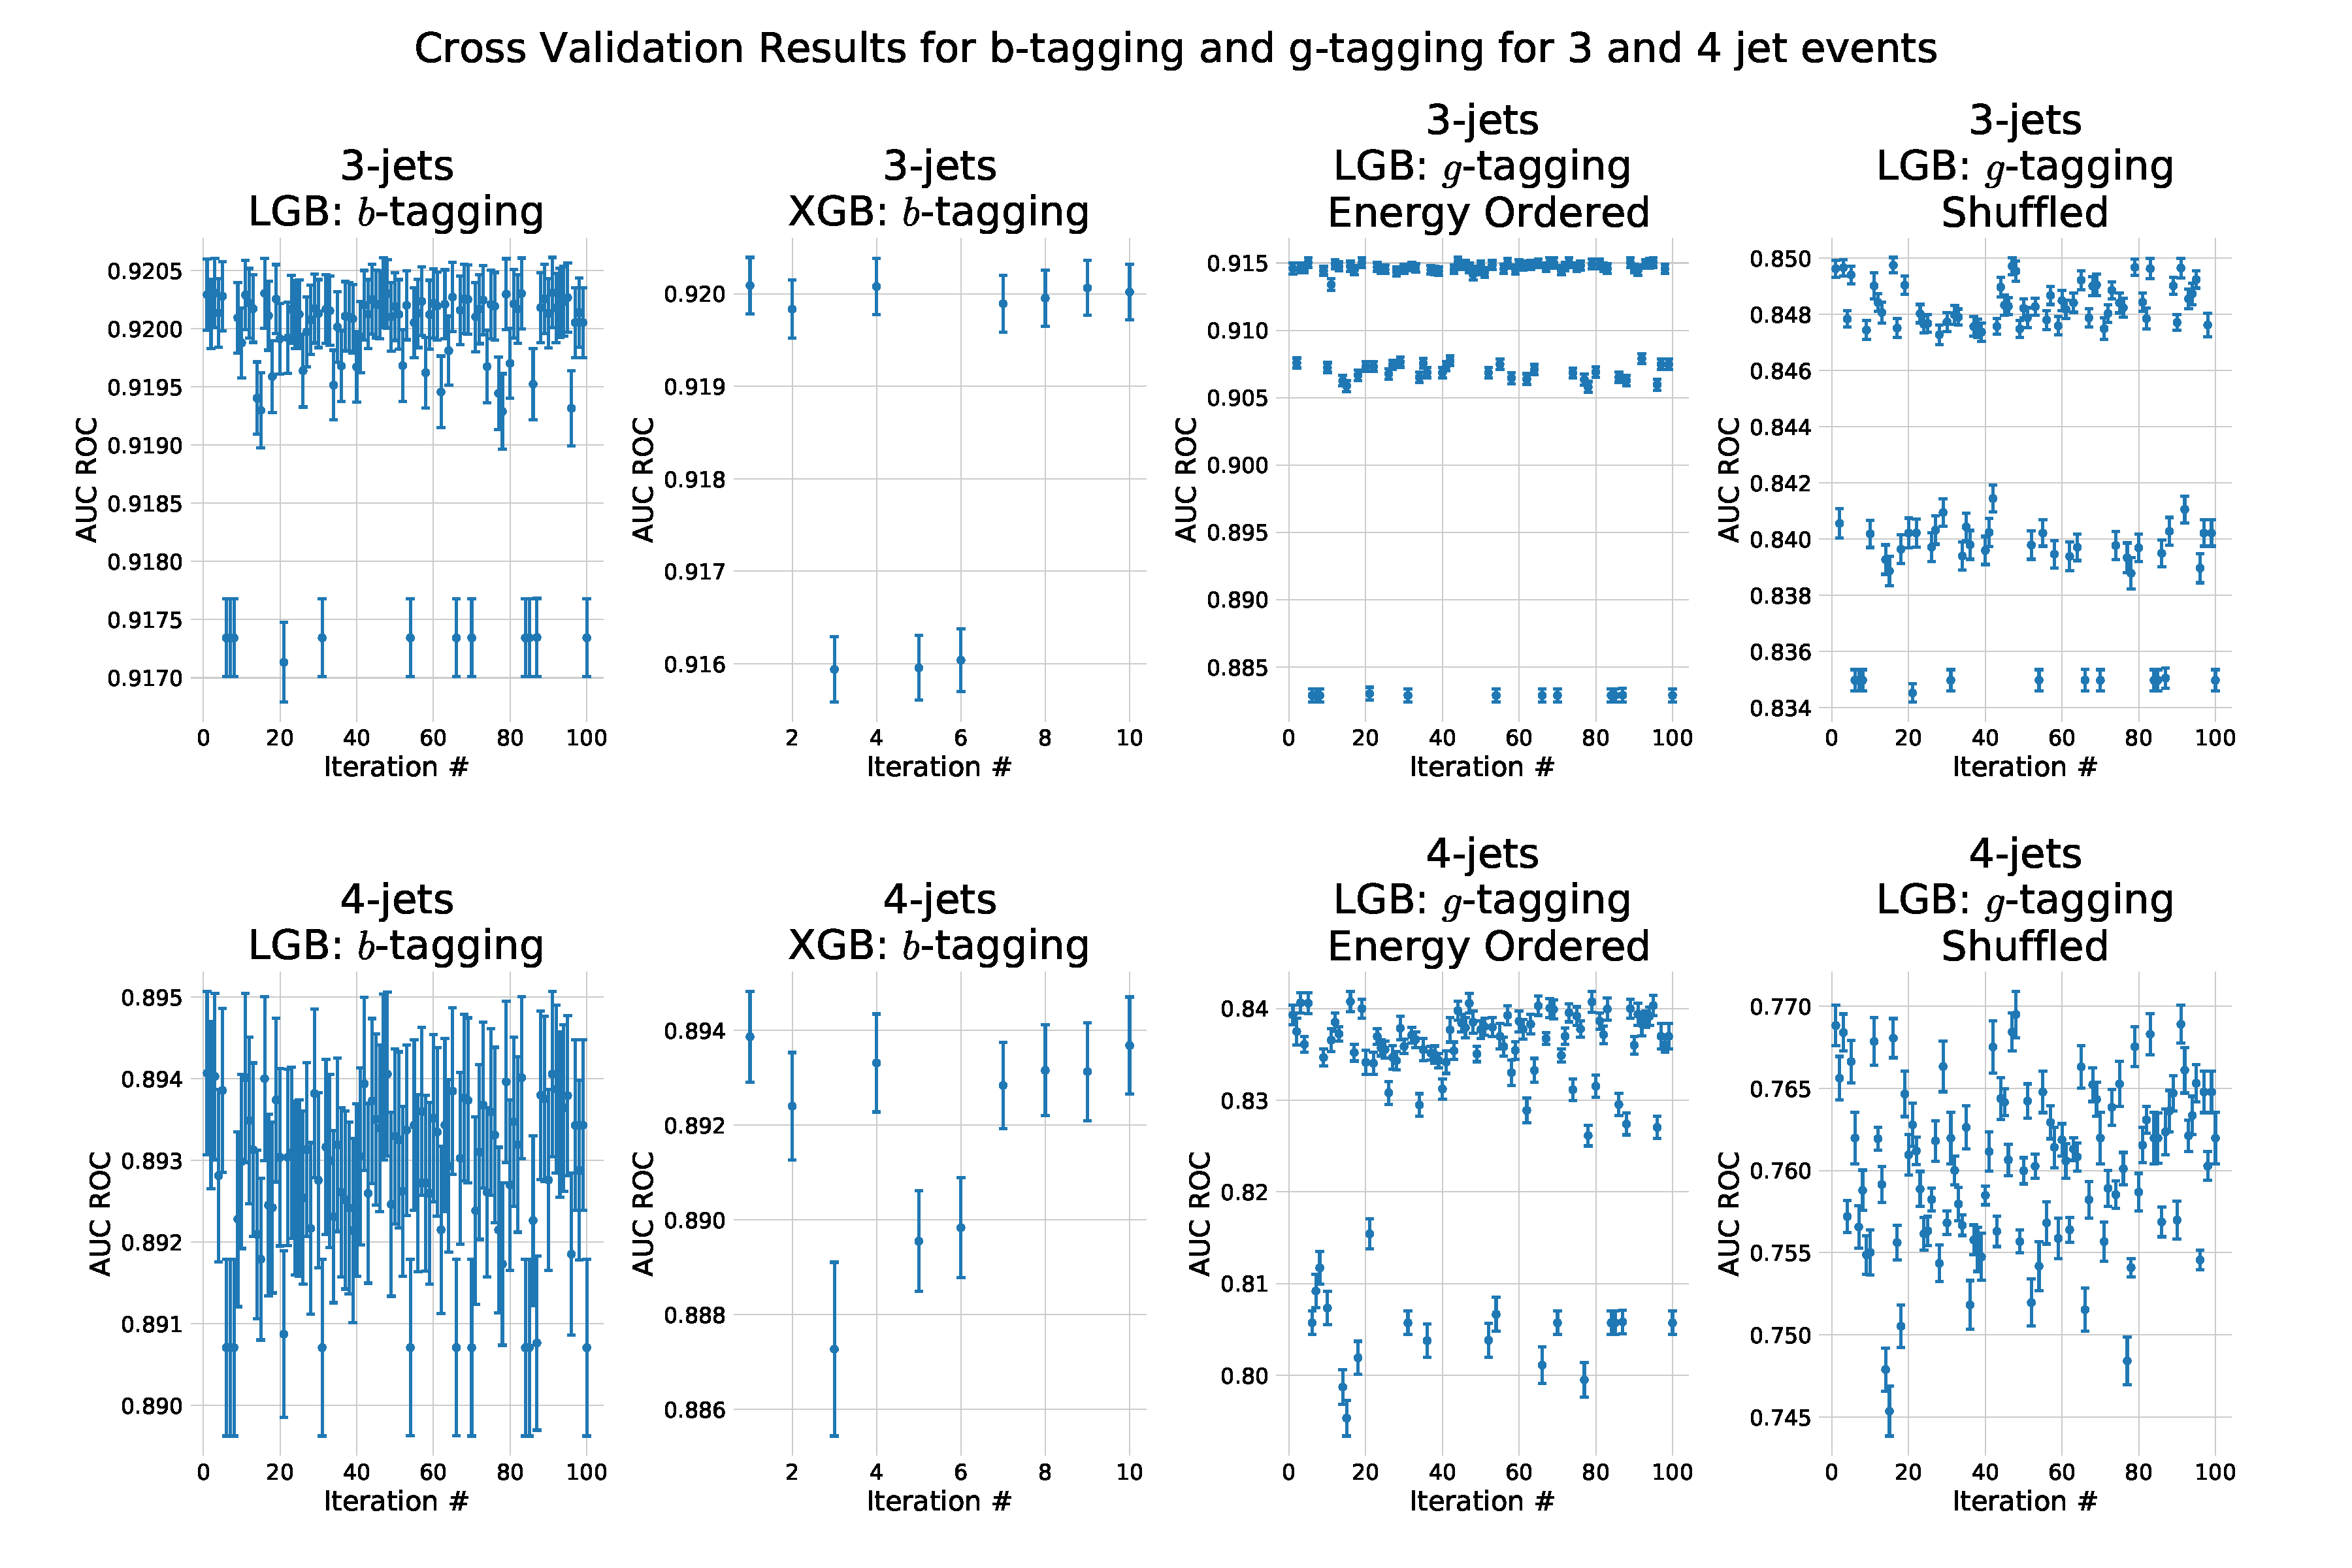
\includegraphics[width=0.95\textwidth, trim=10 10 10 60, clip]{figures/quarks/cv_res_lgb-down_sample=1.00-ML_vars=vertex-selection=b-ejet_min=4-n_iter_RS_lgb=99-n_iter_RS_xgb=9-cdot_cut=0.90-version=19.pdf}
  \caption[Hyperparameter Optimization of b- and g-tagging]
          {Hyperparameter Optimization (HPO) results after running 100 iterations of Random Search (only 10 for XGB). In the top row are the results of the 3-jet models and in the bottom row the results of the 4-jet models. From left to right, we have first) the b-tagging results of XGB, second) the b-tagging results of XGB using only 10 iterations of RS, third) the g-tagging results of XGB fit on the Energy Ordered b-tags, and forth) the g-tagging results of XGB fit on the shuffled b-tags. Notice the different ranges on the y-axes.
          } 
  \label{fig:q:CV_res_iterations}
\end{figure}


\begin{figure}
  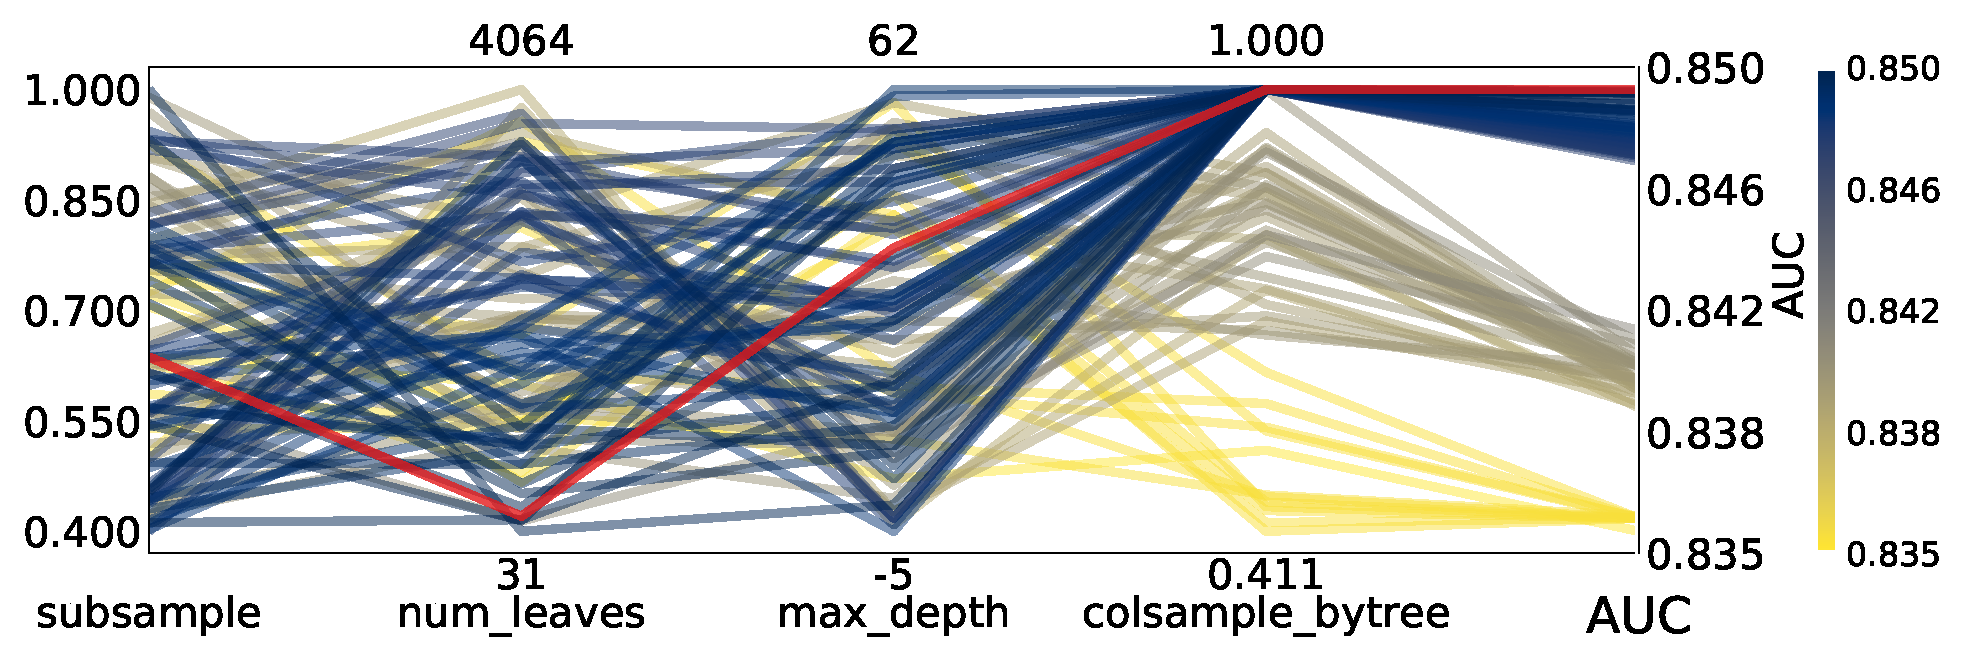
\includegraphics[width=0.95\textwidth, trim=0 0 0 0, clip]{figures/quarks/CV_viz-njet=3-name=lf_gtag_shuffled_lgb_down_sample=1.00-ML_vars=vertex-selection=b-ejet_min=4-n_iter_RS_lgb=99-n_iter_RS_xgb=9-cdot_cut=0.90-version=19.pdf}
  \caption[Overview of Hyperparamaters of g-tagging for 3-jet shuffled events]
          {Hyperparameter optimization results of g-tagging for 3-jet shuffled events. The results are shown as parallel coordinates with each hyperparameter along the x-axis and the value of that parameter on the y-axis. Each line is an event in the 4-dimensional space colored according to the performance of that hyperparameter as measured by AUC from \textcolor{viridis-dark}{highest} AUC in dark blue to \textcolor{viridis-light}{lowest} AUC in yellow. The \textcolor{red}{single best hyperparameter} is shown in red. 
          } 
  \label{fig:q:initial_CV_res_parallel_coords}
\end{figure}



\begin{figure}
  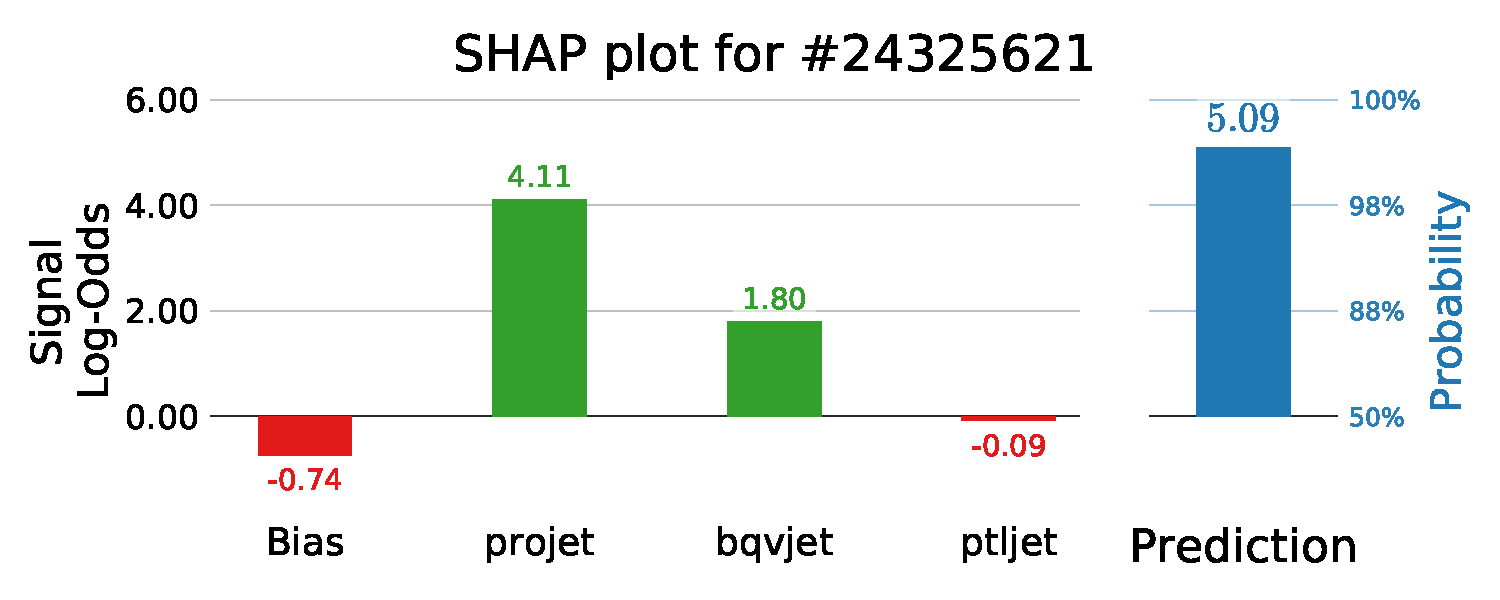
\includegraphics[width=0.95\textwidth, trim=0 0 0 40, clip]{figures/quarks/shap_values-down_sample=1.00-ML_vars=vertex-selection=b-ejet_min=4-n_iter_RS_lgb=99-n_iter_RS_xgb=9-cdot_cut=0.90-version=19-njet=3loc=24325621.pdf}
  \caption[SHAP Prediction Explanation for b-like jet]
          {Model explanation for the 3-jet b-tagging model for a b-like jet. The first column is the bias of the training set which acts as the naive prediction baseline, the rest are the input data variables. On the right hand side of the plot is the model prediction shown. The left part of the plot is shown in log-odds space, the right part in probability space. The model prediction is the sum of the log-odds (5.09 in this example) transformed into probability space. The \textcolor{red}{negative} log-odd values are shown in red, \textcolor{green}{positive} ones in green, and the \textcolor{blue}{prediction value} in blue. 
          } 
  \label{fig:q:shap_signal}
\end{figure}


\begin{figure}
  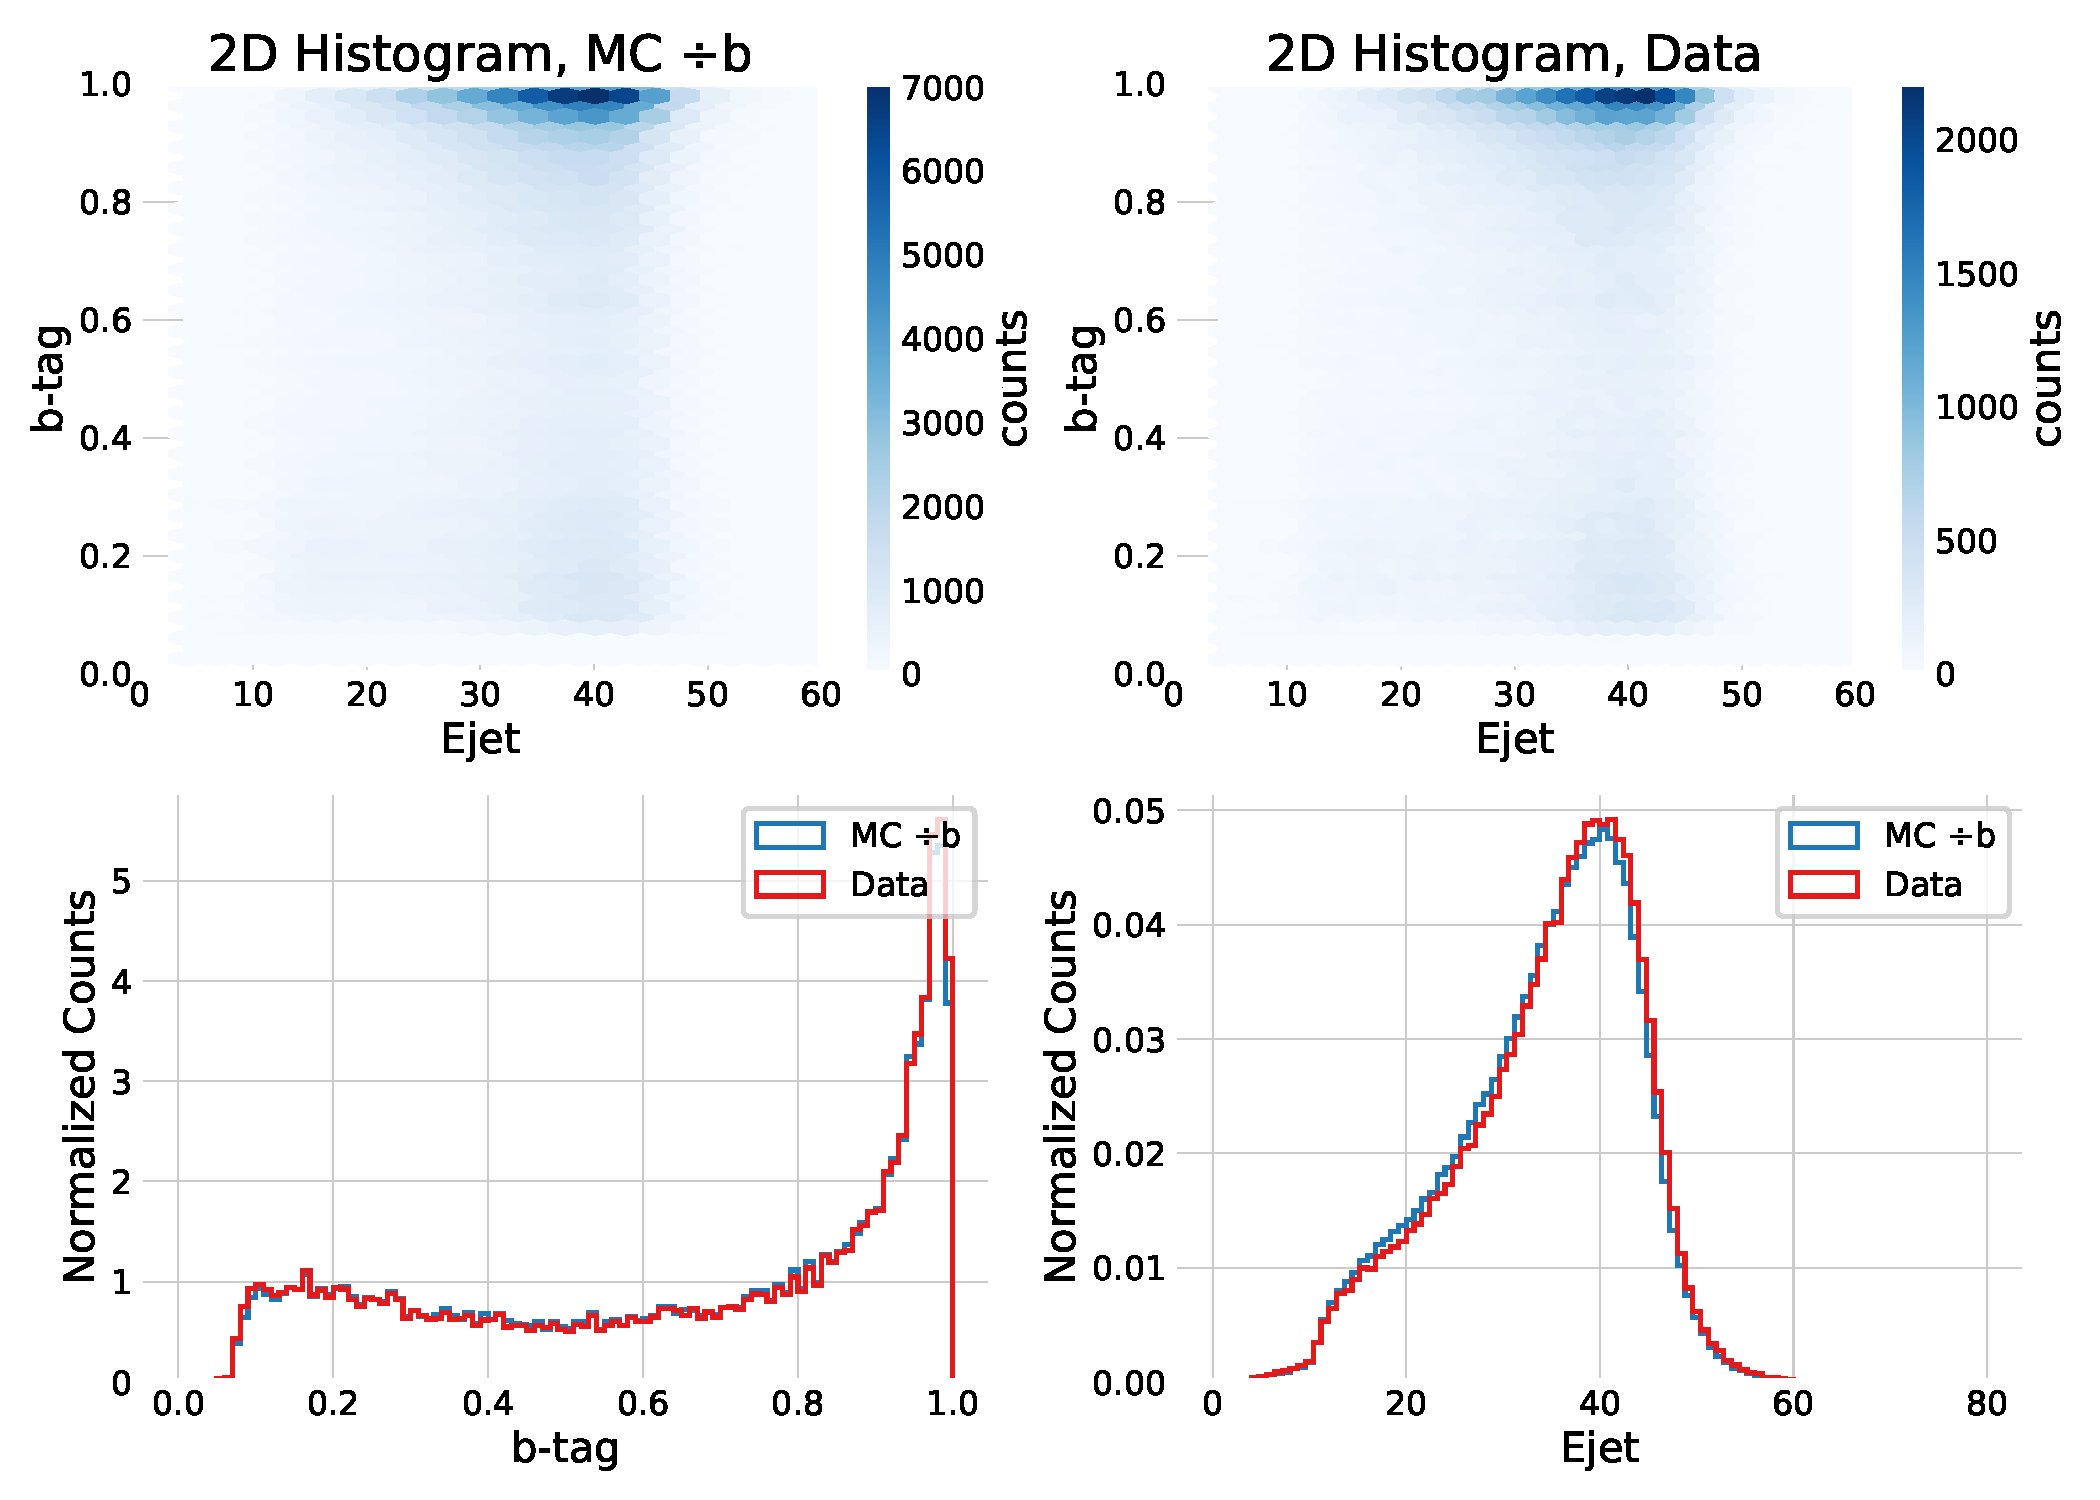
\includegraphics[width=0.95\textwidth, trim=0 0 0 40, clip]{figures/quarks/2d-histograms-ejet-btag-comparison-down_sample=1.00-ML_vars=vertex-selection=b-ejet_min=4-n_iter_RS_lgb=99-n_iter_RS_xgb=9-cdot_cut=0.90-version=19-njet=3.pdf}
  \caption[Monte Carlo -- Data bias for b-tags and jet energy]
          {Comparison of the b-tag and jet energy (\code{Ejet}) distributions for Monte Carlo (MC) versus data. In the top row the 2D-distributions are shown for MC on the left (without the extra MCb samples) and data on the right. In the bottom row the 1D marginal distrubtions are shown for the b-tag and the jet energy with \textcolor{red}{data} in red and \textcolor{blue}{Monte Carlo} ones in blue. Notice the the almost identical distributions in b-tag. 
          } 
  \label{fig:q:btag_Ejet_comparison}
\end{figure}

\begin{figure}
  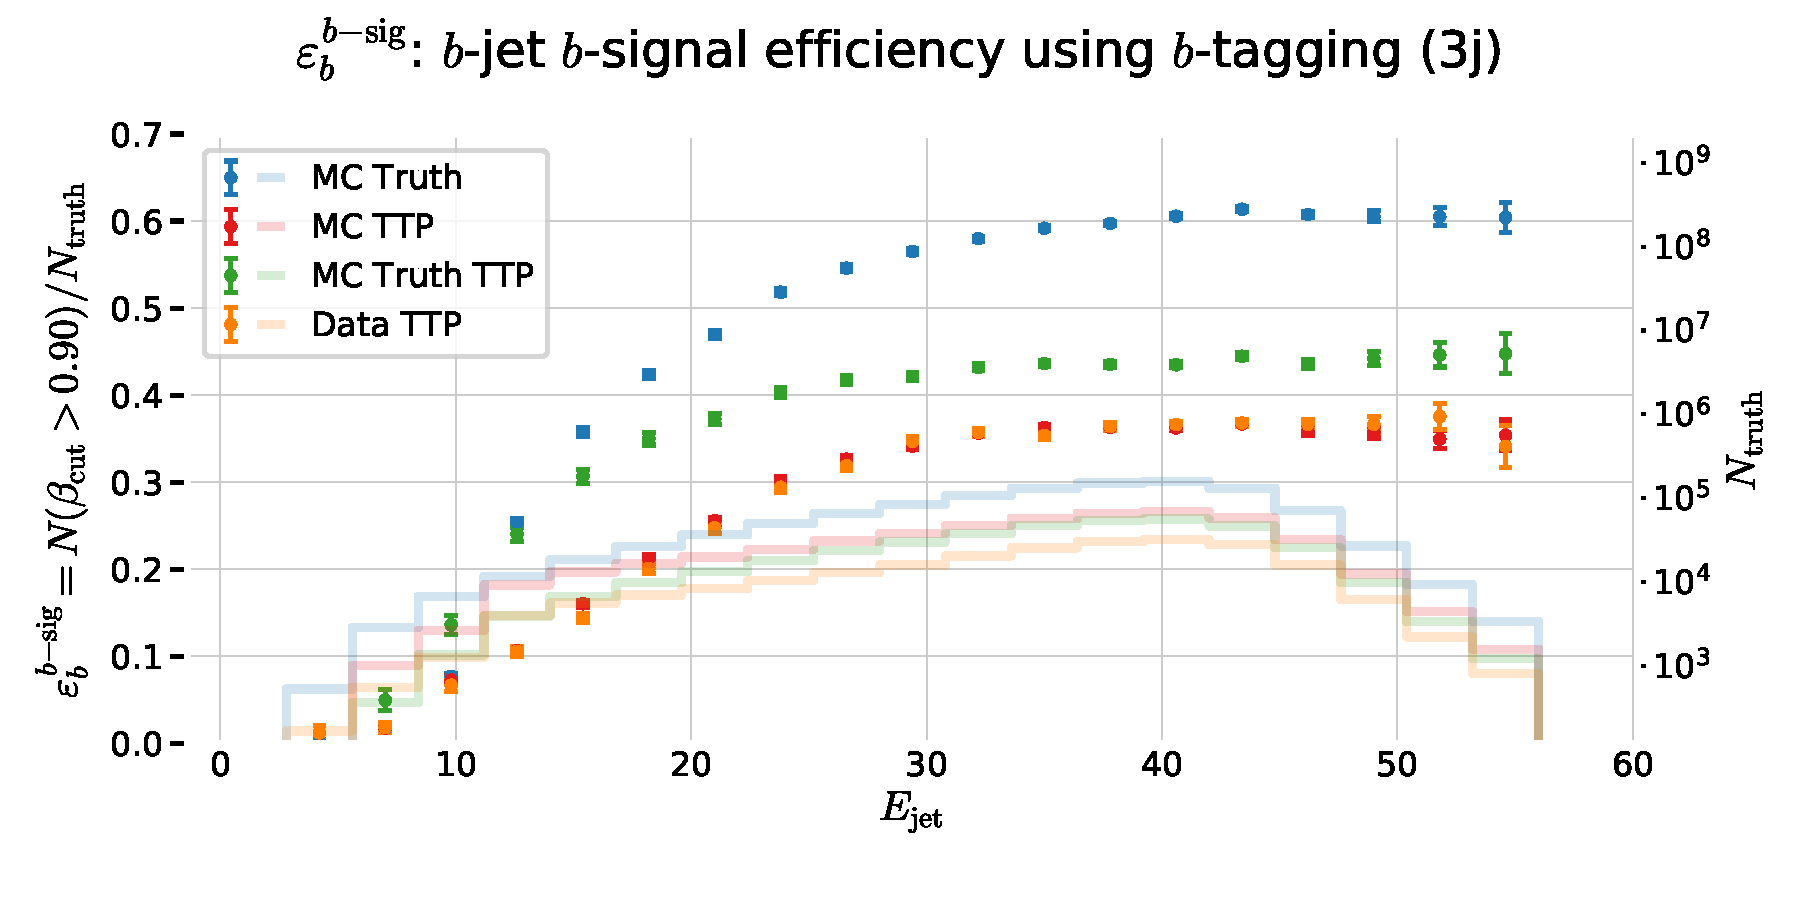
\includegraphics[width=0.95\textwidth, trim=0 0 0 40, clip]{figures/quarks/eff_b_bsig-down_sample=1.00-ML_vars=vertex-selection=b-ejet_min=4-n_iter_RS_lgb=99-n_iter_RS_xgb=9-cdot_cut=0.90-version=19.pdf}
  \caption[b-Tagging Efficiency $\varepsilon_b^{b\mathrm{-sig}}$ as a function of jet energy]
          {Efficiency of the b-tags for b-jets in the b-signal region for 3-jet events, $\varepsilon_b^{b\mathrm{-sig}}$, as a function of jet energy \code{Ejet}. The b-signal region is defined as $\beta > 0.9$. In the plot the efficiencies are shown for \textcolor{blue}{MC Truth} in blue, \textcolor{red}{MC TTP} in red, \textcolor{green}{MC Truth TTP} in green, and \textcolor{orange}{Data TTP} in orange. The efficiencies (the errorbars) can be read off on the left y-axis and the counts (histograms) on the right y-axis. The abbreviation TTP is short for \q{Tag, Tag, Probe} where two jets in a event are used as tags and the probe is then used for further analysis. Notice how both MC TTP and Data TTP follow each other closely.  
          } 
  \label{fig:q:effiency_btag_bjet_bsig}
\end{figure}


\begin{figure}
  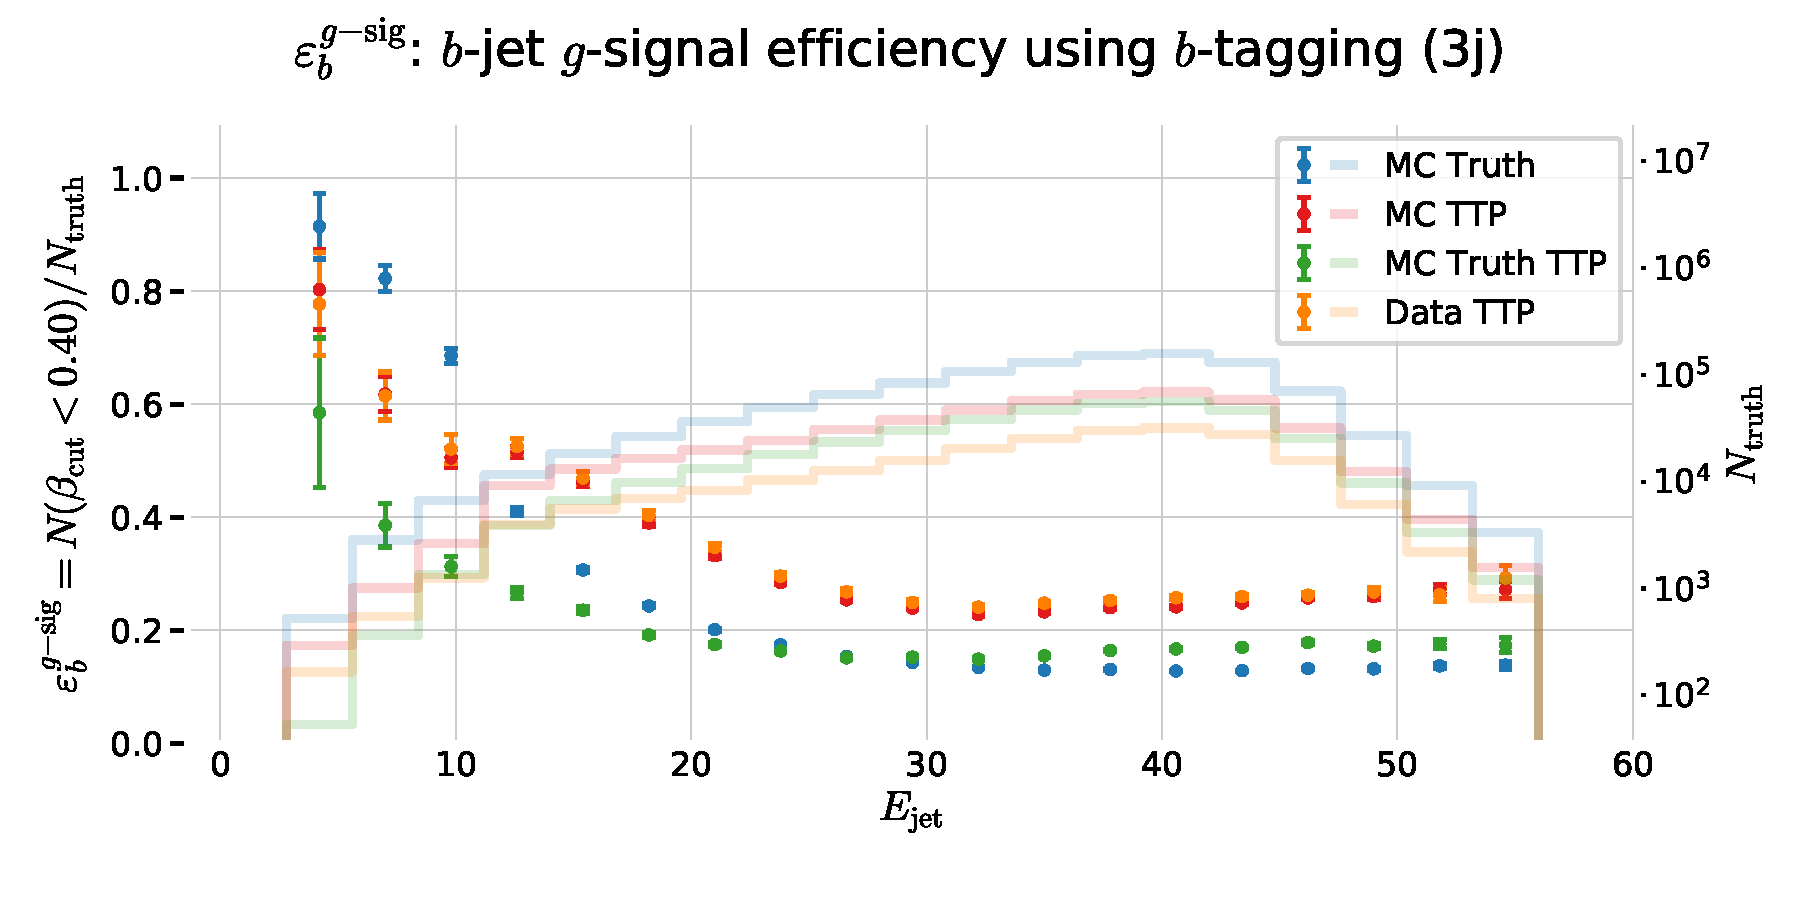
\includegraphics[width=0.95\textwidth, trim=0 0 0 40, clip]{figures/quarks/eff_b_gsig-down_sample=1.00-ML_vars=vertex-selection=b-ejet_min=4-n_iter_RS_lgb=99-n_iter_RS_xgb=9-cdot_cut=0.90-version=19.pdf}
  \caption[b-Tagging Efficiency $\varepsilon_b^{g\mathrm{-sig}}$ as a function of jet energy]
          {Efficiency of the b-tags for b-jets in the g-signal region for 3-jet events, $\varepsilon_b^{g\mathrm{-sig}}$, as a function of jet energy \code{Ejet}. The g-signal region is defined as $\beta < 0.4$. In the plot the efficiencies are shown for \textcolor{blue}{MC Truth} in blue, \textcolor{red}{MC TTP} in red, \textcolor{green}{MC Truth TTP} in green, and \textcolor{orange}{Data TTP} in orange. The efficiencies (the errorbars) can be read off on the left y-axis and the counts (histograms) on the right y-axis. The abbreviation TTP is short for \q{Tag, Tag, Probe} where two jets in a event are used as tags and the probe is then used for further analysis. Notice how both MC TTP and Data TTP follow each other closely.  
          } 
  \label{fig:q:effiency_btag_bjet_gsig}
\end{figure}


\begin{figure}
  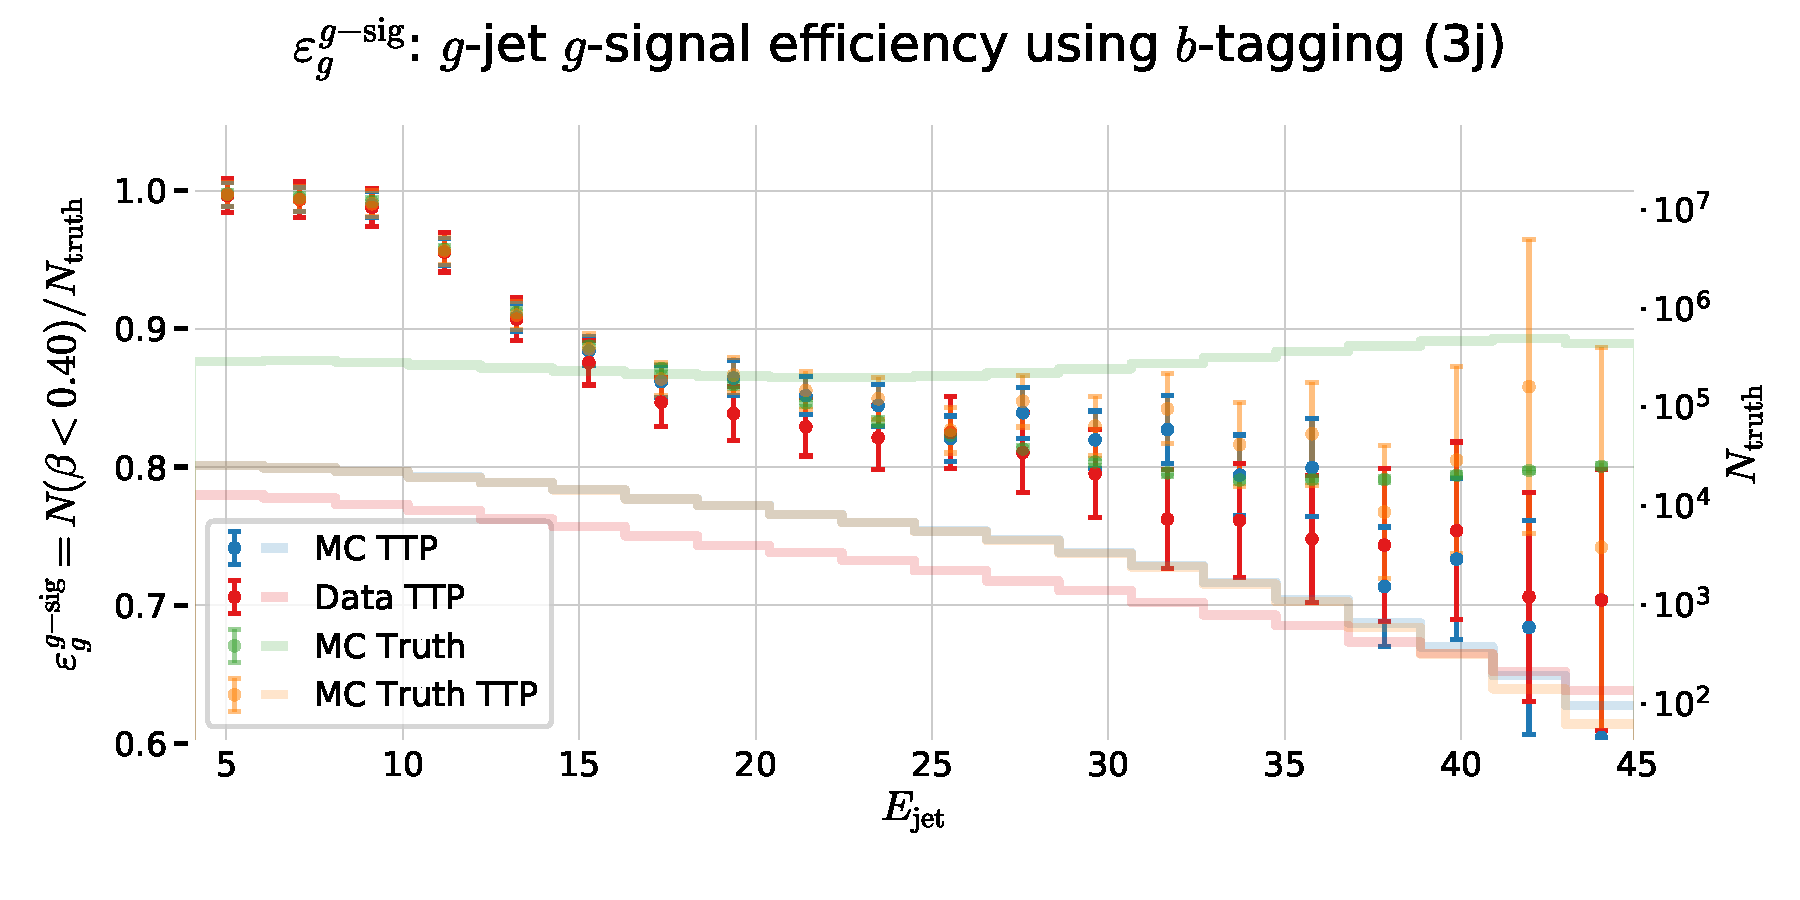
\includegraphics[width=0.95\textwidth, trim=0 0 0 40, clip]{figures/quarks/eff_g_gsig-down_sample=1.00-ML_vars=vertex-selection=b-ejet_min=4-n_iter_RS_lgb=99-n_iter_RS_xgb=9-cdot_cut=0.90-version=19.pdf}
  \caption[b-Tagging Efficiency $\varepsilon_g^{g\mathrm{-sig}}$ as a function of jet energy]
          {Efficiency of the b-tags for g-jets in the g-signal region for 3-jet events, $\varepsilon_g^{g\mathrm{-sig}}$, as a function of jet energy \code{Ejet}. The g-signal region is defined as $\beta < 0.4$. In the plot the efficiencies are shown for \textcolor{blue}{MC Truth} in blue, \textcolor{red}{MC TTP} in red, \textcolor{green}{MC Truth TTP} in green, and \textcolor{orange}{Data TTP} in orange. The efficiencies (the errorbars) can be read off on the left y-axis and the counts (histograms) on the right y-axis. The abbreviation TTP is short for \q{Tag, Tag, Probe} where two jets in a event are used as tags and the probe is then used for further analysis. Notice how both MC TTP and Data TTP follow each other closely.  
          } 
  \label{fig:q:effiency_btag_gjet_gsig}
\end{figure}

\begin{figure}
  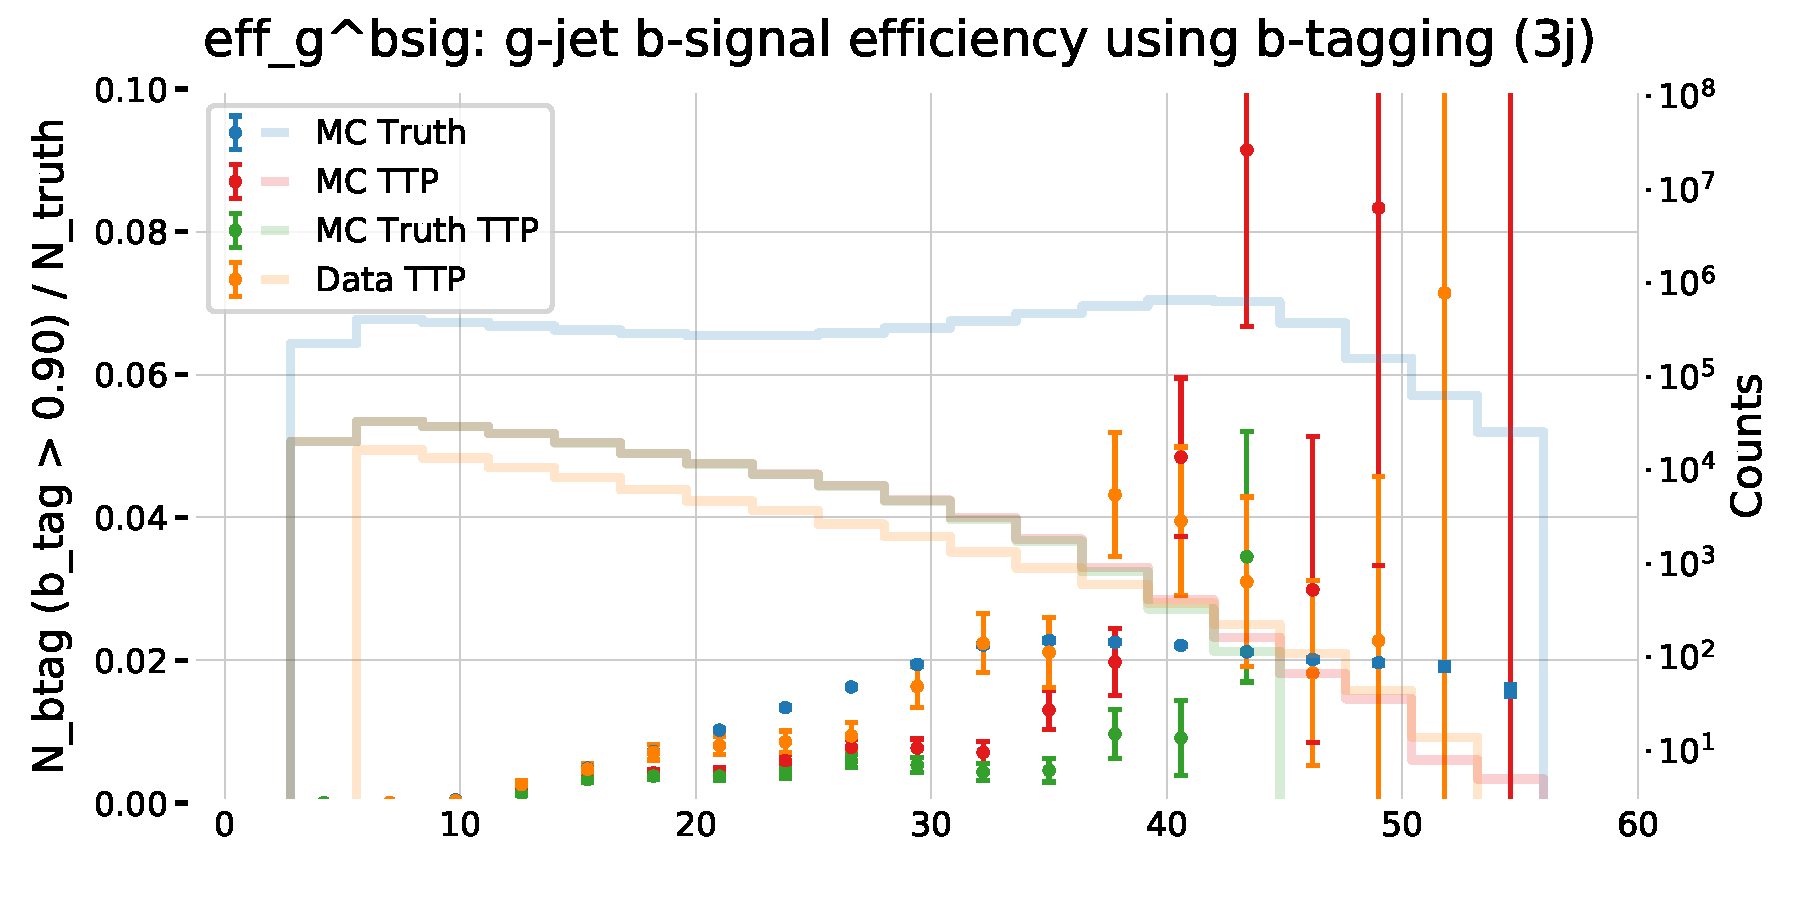
\includegraphics[width=0.95\textwidth, trim=0 0 0 30, clip]{figures/quarks/eff_g_bsig-down_sample=1.00-ML_vars=vertex-selection=b-ejet_min=4-n_iter_RS_lgb=99-n_iter_RS_xgb=9-cdot_cut=0.90-version=19.pdf}
  \caption[b-Tagging Efficiency $\varepsilon_g^{b\mathrm{-sig}}$ as a function of jet energy]
          {Efficiency of the b-tags for g-jets in the b-signal region for 3-jet events, $\varepsilon_g^{b\mathrm{-sig}}$, as a function of jet energy \code{Ejet}. The b-signal region is defined as $\beta > 0.9$. In the plot the efficiencies are shown for \textcolor{blue}{MC Truth} in blue, \textcolor{red}{MC TTP} in red, \textcolor{green}{MC Truth TTP} in green, and \textcolor{orange}{Data TTP} in orange. The efficiencies (the errorbars) can be read off on the left y-axis and the counts (histograms) on the right y-axis. The abbreviation TTP is short for \q{Tag, Tag, Probe} where two jets in a event are used as tags and the probe is then used for further analysis.  
          } 
  \label{fig:q:effiency_btag_gjet_bsig}
\end{figure}


\begin{figure}
  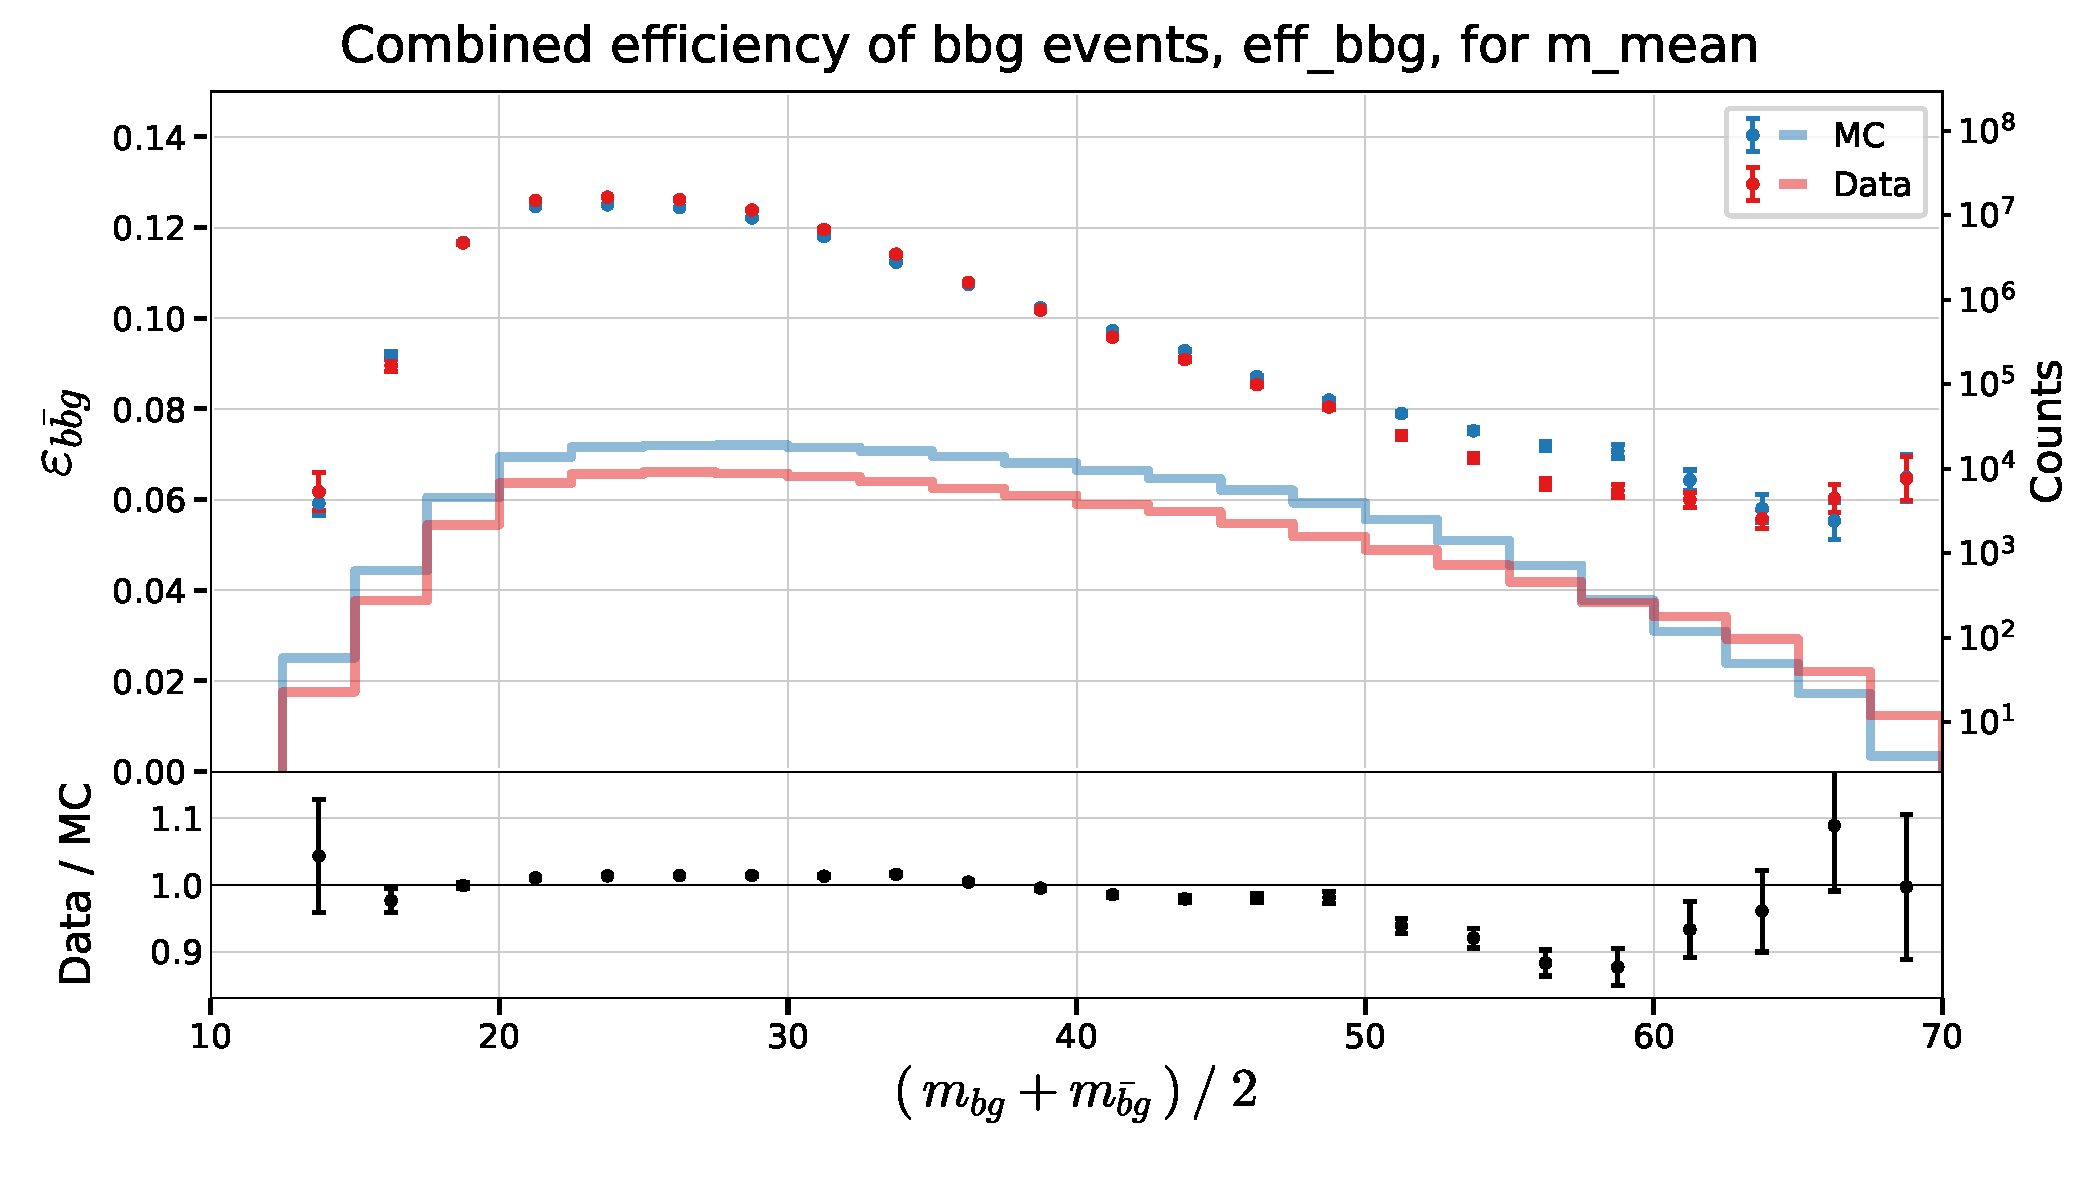
\includegraphics[width=0.95\textwidth, trim=0 0 0 40, clip]{figures/quarks/eff_bbg_m_mean-down_sample=1.00-ML_vars=vertex-selection=b-ejet_min=4-n_iter_RS_lgb=99-n_iter_RS_xgb=9-cdot_cut=0.90-version=19.pdf}
  \caption[g-Tagging proxy efficiency for $b\bar{b}g$-events as function of the mean invariant mass]
          {Proxy efficiency of the g-tags for $b\bar{b}g$ 3-jet events as a function of the mean of the two invariant masses $m_{bg}$ and $m_{\bar{b}g}$. The proxy efficiency $\varepsilon_{b\bar{b}g}$ is measured by finding $b\bar{b}g$-events where $\beta_b > 0.9$, $\beta_{\bar{b}}>0.9$, and $\beta_g < 0.4$. and then calculating  $\varepsilon_{b\bar{b}g} = \varepsilon_b^{b\mathrm{-sig}} \cdot \varepsilon_{\bar{b}}^{b\mathrm{-sig}} \cdot  \varepsilon_g^{g\mathrm{-sig}} $. In the top plot $\varepsilon_{b\bar{b}g}$ is shown for \textcolor{blue}{MC} in blue and \textcolor{red}{Data} in red where the counts in each bin can be read on right y-axis. In the bottom plot the ratio between Data and MC is shown.
          } 
  \label{fig:q:effiency_btag_bbg_m_mean}
\end{figure}


\begin{figure}
  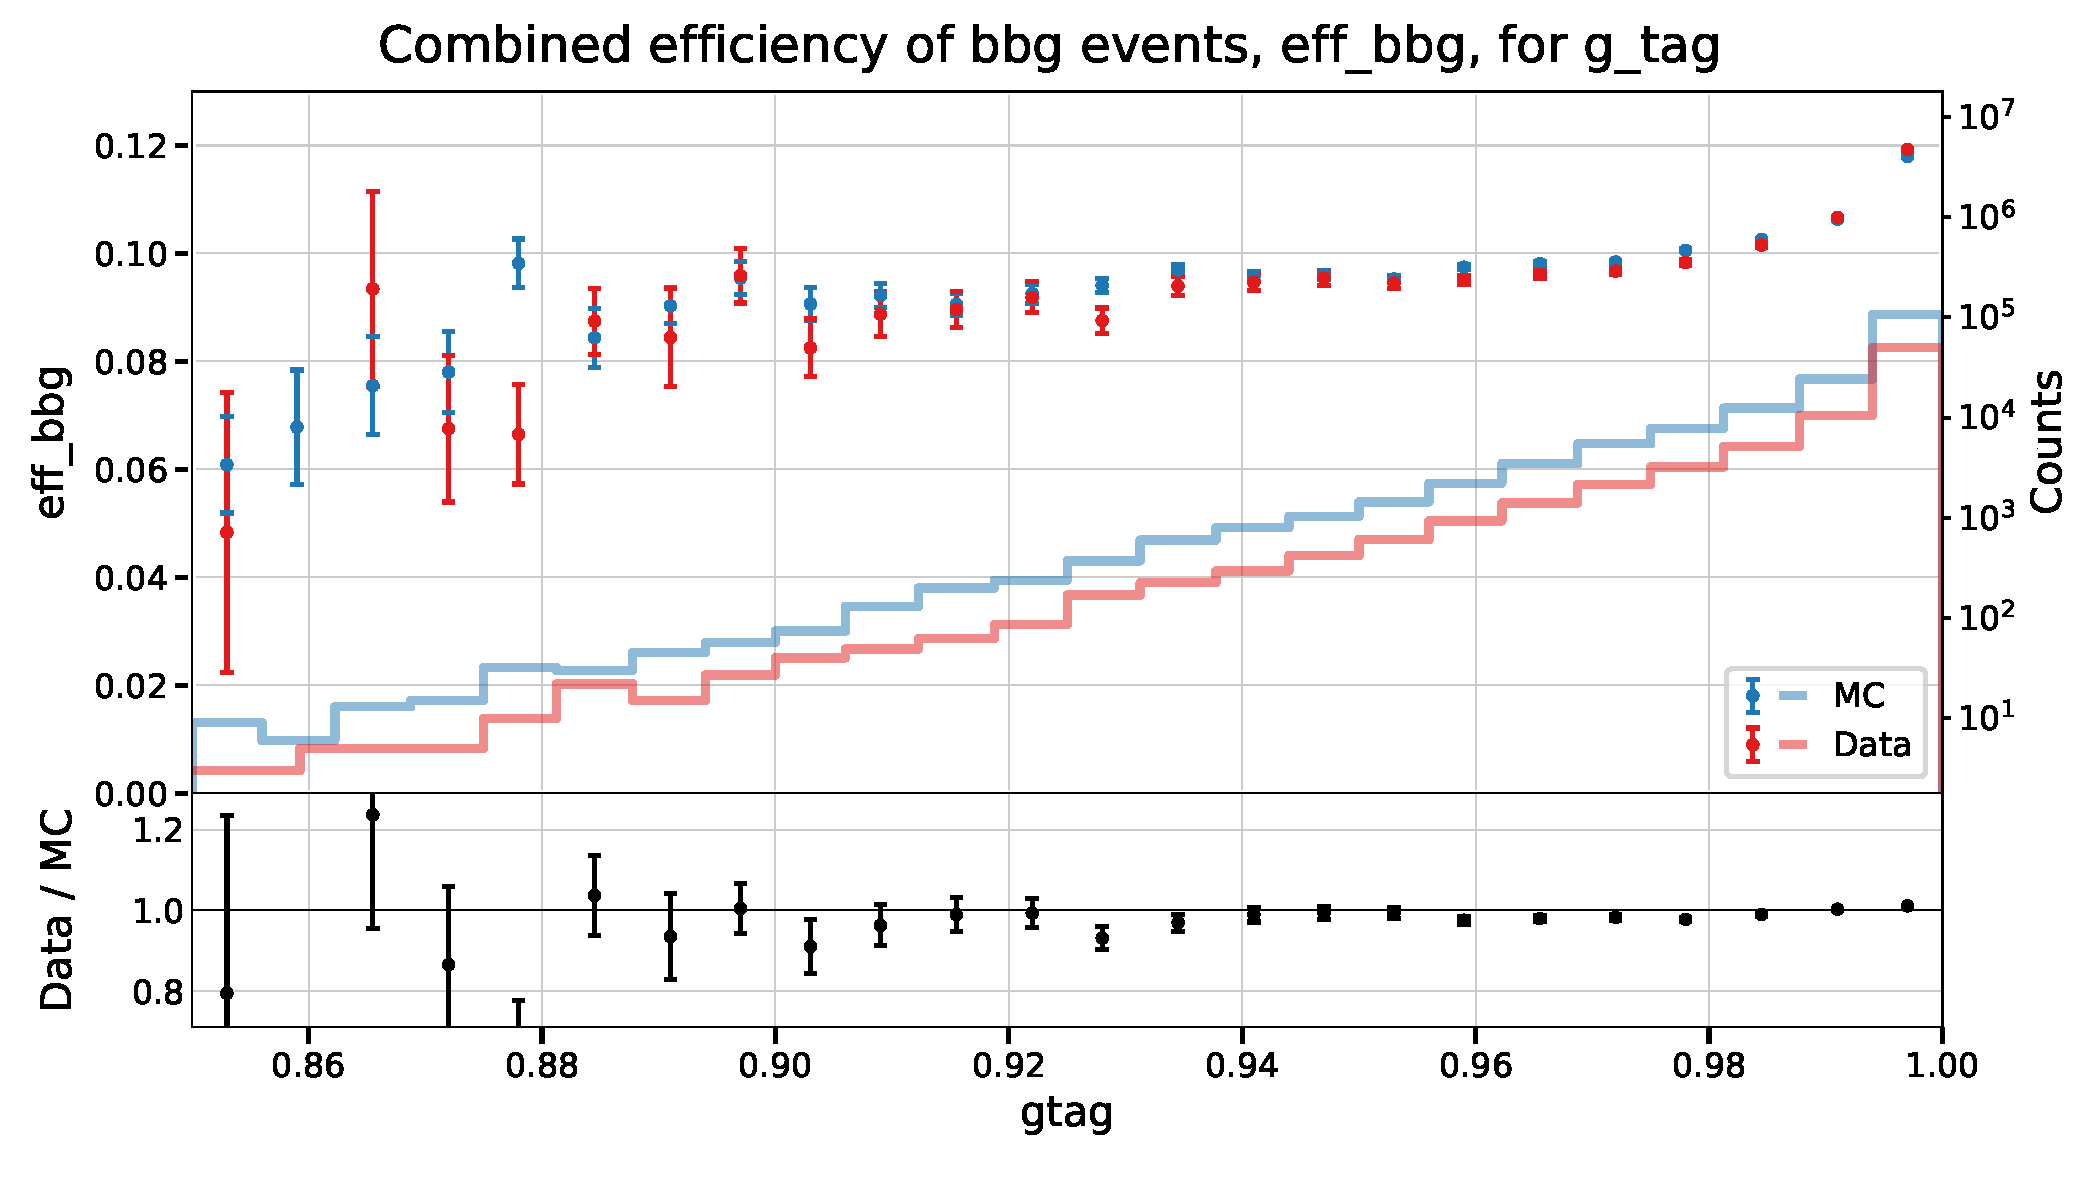
\includegraphics[width=0.95\textwidth, trim=0 0 0 40, clip]{figures/quarks/eff_bbg_gtag-down_sample=1.00-ML_vars=vertex-selection=b-ejet_min=4-n_iter_RS_lgb=99-n_iter_RS_xgb=9-cdot_cut=0.90-version=19.pdf}
  \caption[g-Tagging proxy efficiency for $b\bar{b}g$-events as function of g-tag]
          {Proxy efficiency of the g-tags for $b\bar{b}g$ 3-jet events as a function of the event's g-tag. The proxy efficiency $\varepsilon_{b\bar{b}g}$ is measured by finding $b\bar{b}g$-events where $\beta_b > 0.9$, $\beta_{\bar{b}}>0.9$, and $\beta_g < 0.4$. and then calculating  $\varepsilon_{b\bar{b}g} = \varepsilon_b^{b\mathrm{-sig}} \cdot \varepsilon_{\bar{b}}^{b\mathrm{-sig}} \cdot  \varepsilon_g^{g\mathrm{-sig}} $. In the top plot $\varepsilon_{b\bar{b}g}$ is shown for \textcolor{blue}{MC} in blue and \textcolor{red}{Data} in red where the counts in each bin can be read on right y-axis. In the bottom plot the ratio between Data and MC is shown.
          } 
  \label{fig:q:effiency_btag_bbg_gtag}
\end{figure}



\begin{figure}
  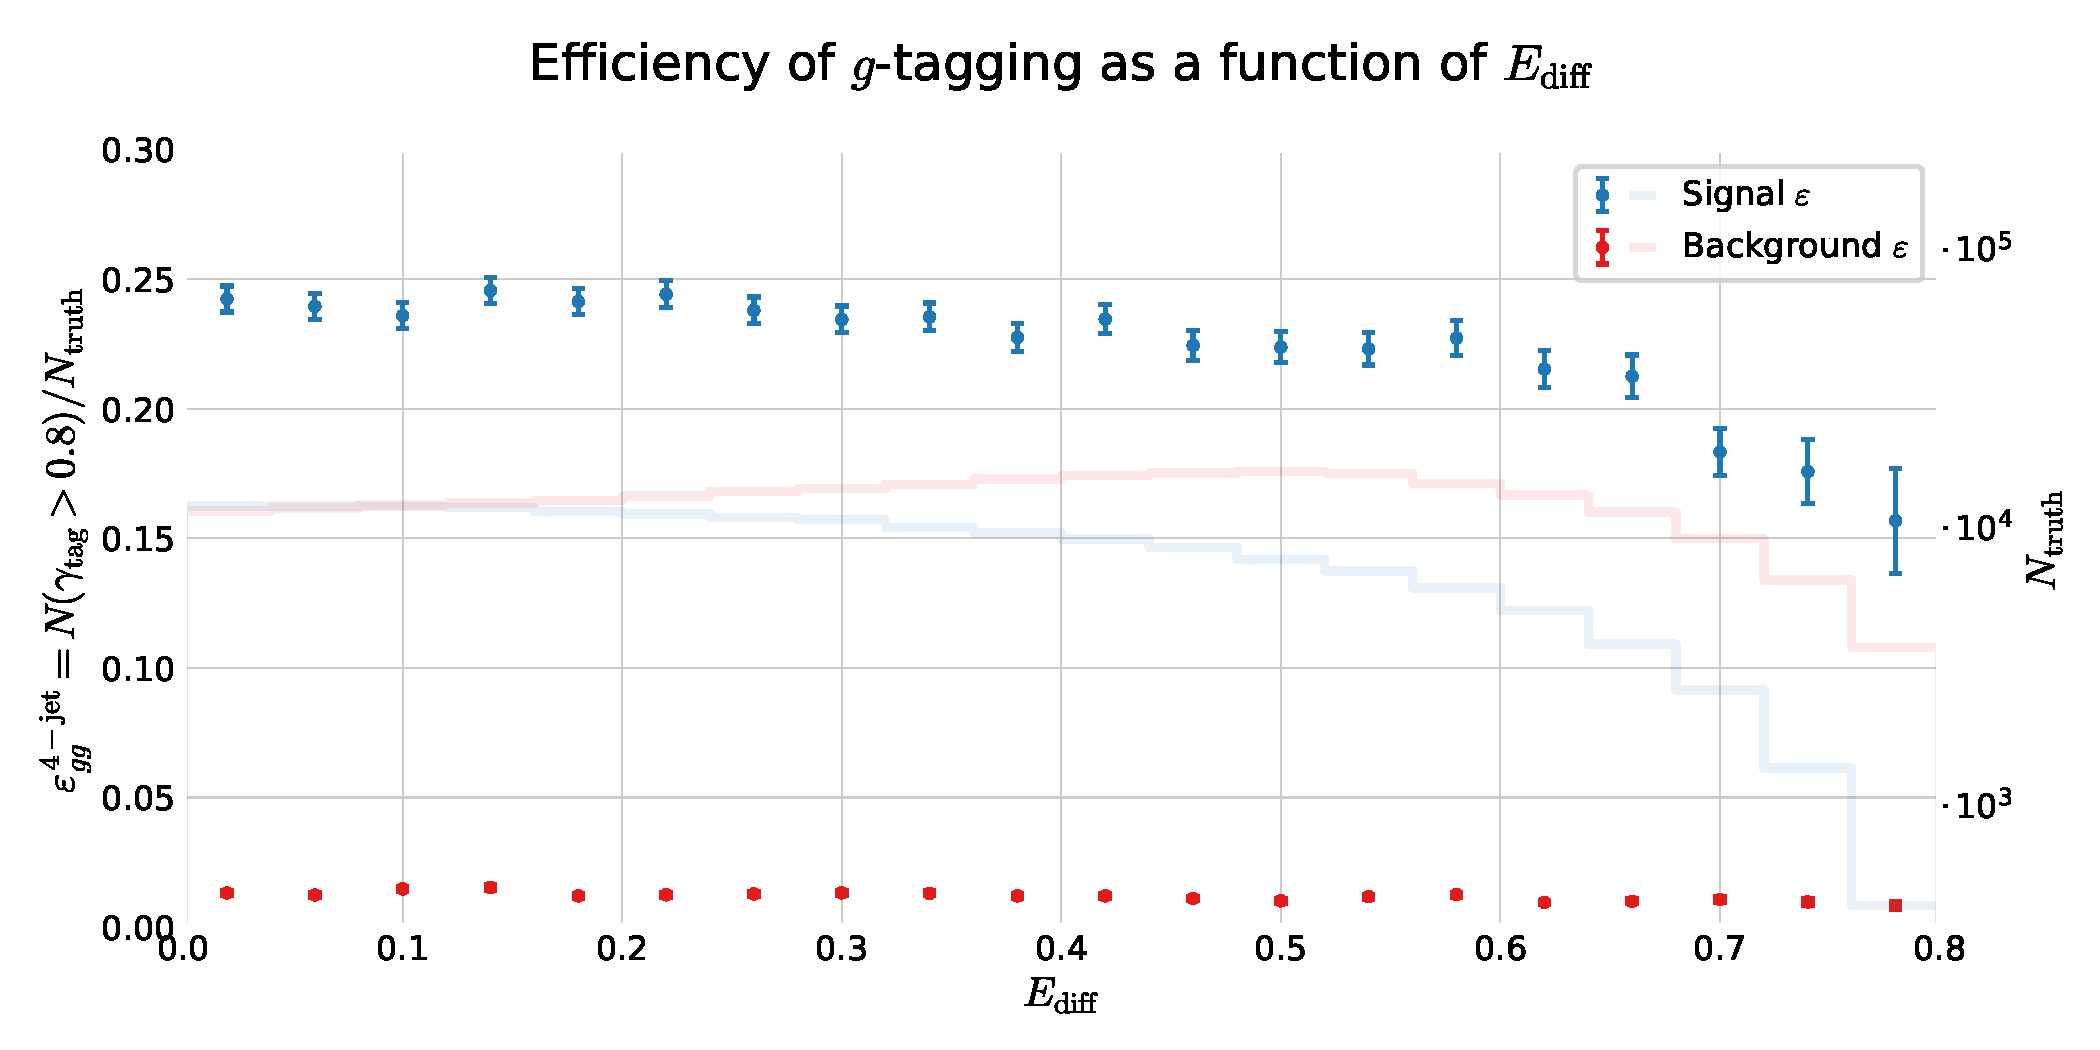
\includegraphics[width=0.95\textwidth, trim=0 0 0 40, clip, page=1]{figures/quarks/efficiency_events-down_sample=1.00-ML_vars=vertex-selection=b-ejet_min=4-n_iter_RS_lgb=99-n_iter_RS_xgb=9-cdot_cut=0.90-version=19-njet=4.pdf}
  \caption[g-Tagging efficiency for 4-jet events in MC as a function of normalized gluon gluon jet energy difference]
          {Efficiency of the g-tags for 4-jet events as a function of normalized gluon gluon jet energy difference in Monte Carlo. The efficiency is measured as the number of events with a g-tag higher than 0.8 ($\gamma > 0.8$) out of the total number and the normalized gluon gluon jet energy difference $A$ is $A=\frac{E_{g_\mathrm{max}}-E_{g_\mathrm{min}}}{E_{g_\mathrm{max}}+E_{g_\mathrm{min}}}$ where $E_{g_\mathrm{max}}$ ($E_{g_\mathrm{min}}$) refers to the energy of the gluon with the highest (lowest) energy. The efficiency is plotted for \textcolor{blue}{signal events} according to MC Truth in blue and \textcolor{red}{background events} according to MC Truth in red.
          } 
  \label{fig:q:effiency_gtag_E_diff}
\end{figure}


\begin{figure}
  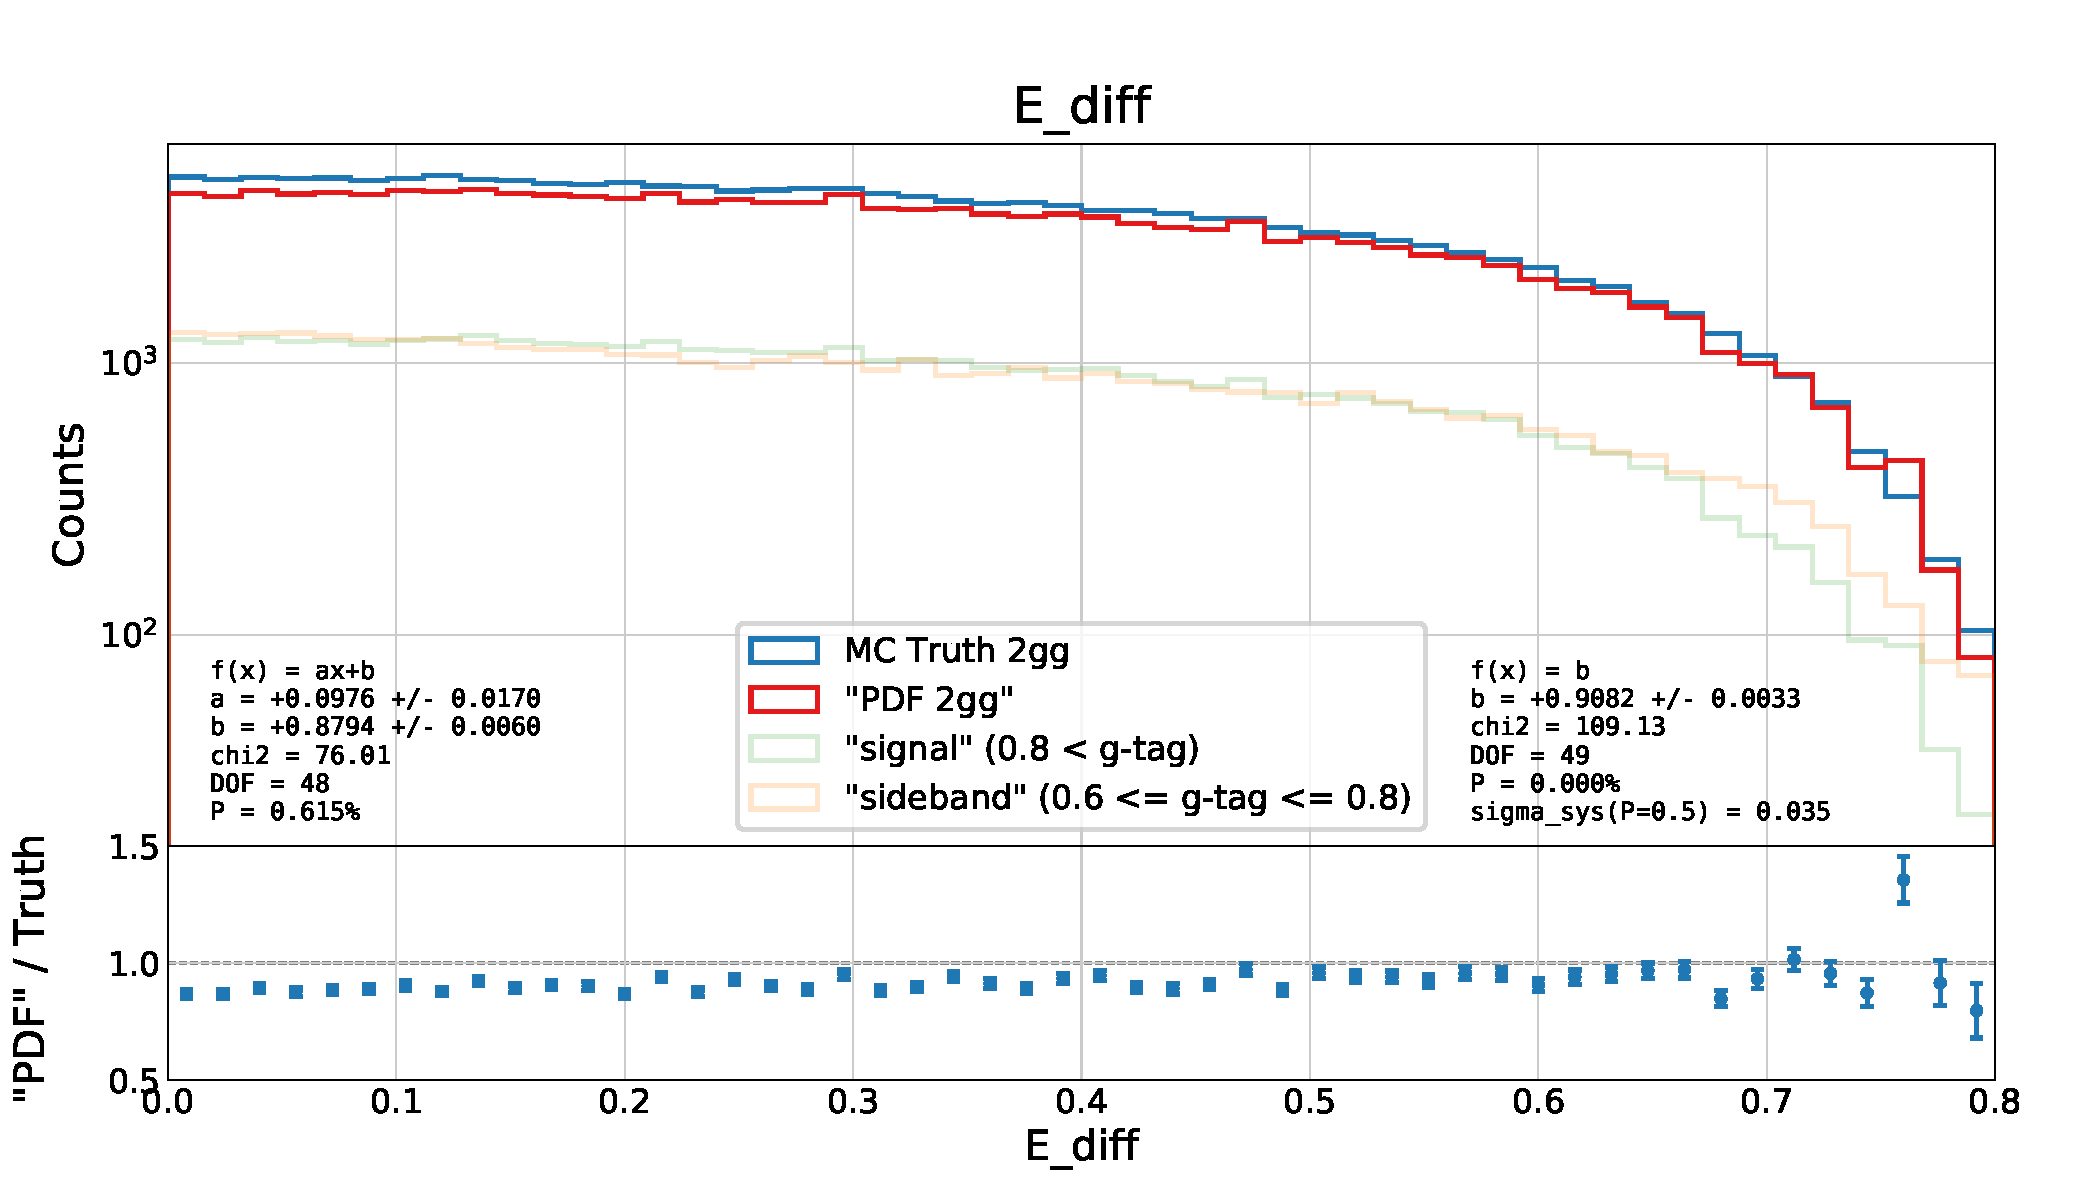
\includegraphics[width=0.95\textwidth, trim=0 0 0 65, clip, page=1]{figures/quarks/gtag-closure_test-down_sample=1.00-ML_vars=vertex-selection=b-ejet_min=4-n_iter_RS_lgb=99-n_iter_RS_xgb=9-cdot_cut=0.90-version=19-njet=3.pdf}
  \caption[Closure plot between MC Truth and the corrected g-tagging model in 4-jet events for the normalized gluon gluon jet energy difference]
          {Closure plot between MC Truth and the corrected g-tagging model in 4-jet events for the normalized gluon gluon jet energy difference. The corrected g-taggingg model is described in further detail in section XXX \TODO. In the top part of the plot the \textcolor{blue}{MC Truth} is shown in blue, the \textcolor{red}{corrected g-tagging model} \code{"PDF 2gg"} in red, the \textcolor{green}{g-signal distribution} in semi-transparent green and the \textcolor{orange}{g-sideband distribution} in semi-transparent orange. In the bottom part of the plot the ratio between MC Truth and the output of the corrected g-tagging model is shown. The normalized gluon gluon jet energy difference $A$ is $A=\frac{E_{g_\mathrm{max}}-E_{g_\mathrm{min}}}{E_{g_\mathrm{max}}+E_{g_\mathrm{min}}}$ where $E_{g_\mathrm{max}}$ ($E_{g_\mathrm{min}}$) refers to the energy of the gluon with the highest (lowest) energy.
          } 
  \label{fig:q:closure_E_diff}
\end{figure}


\begin{figure}
  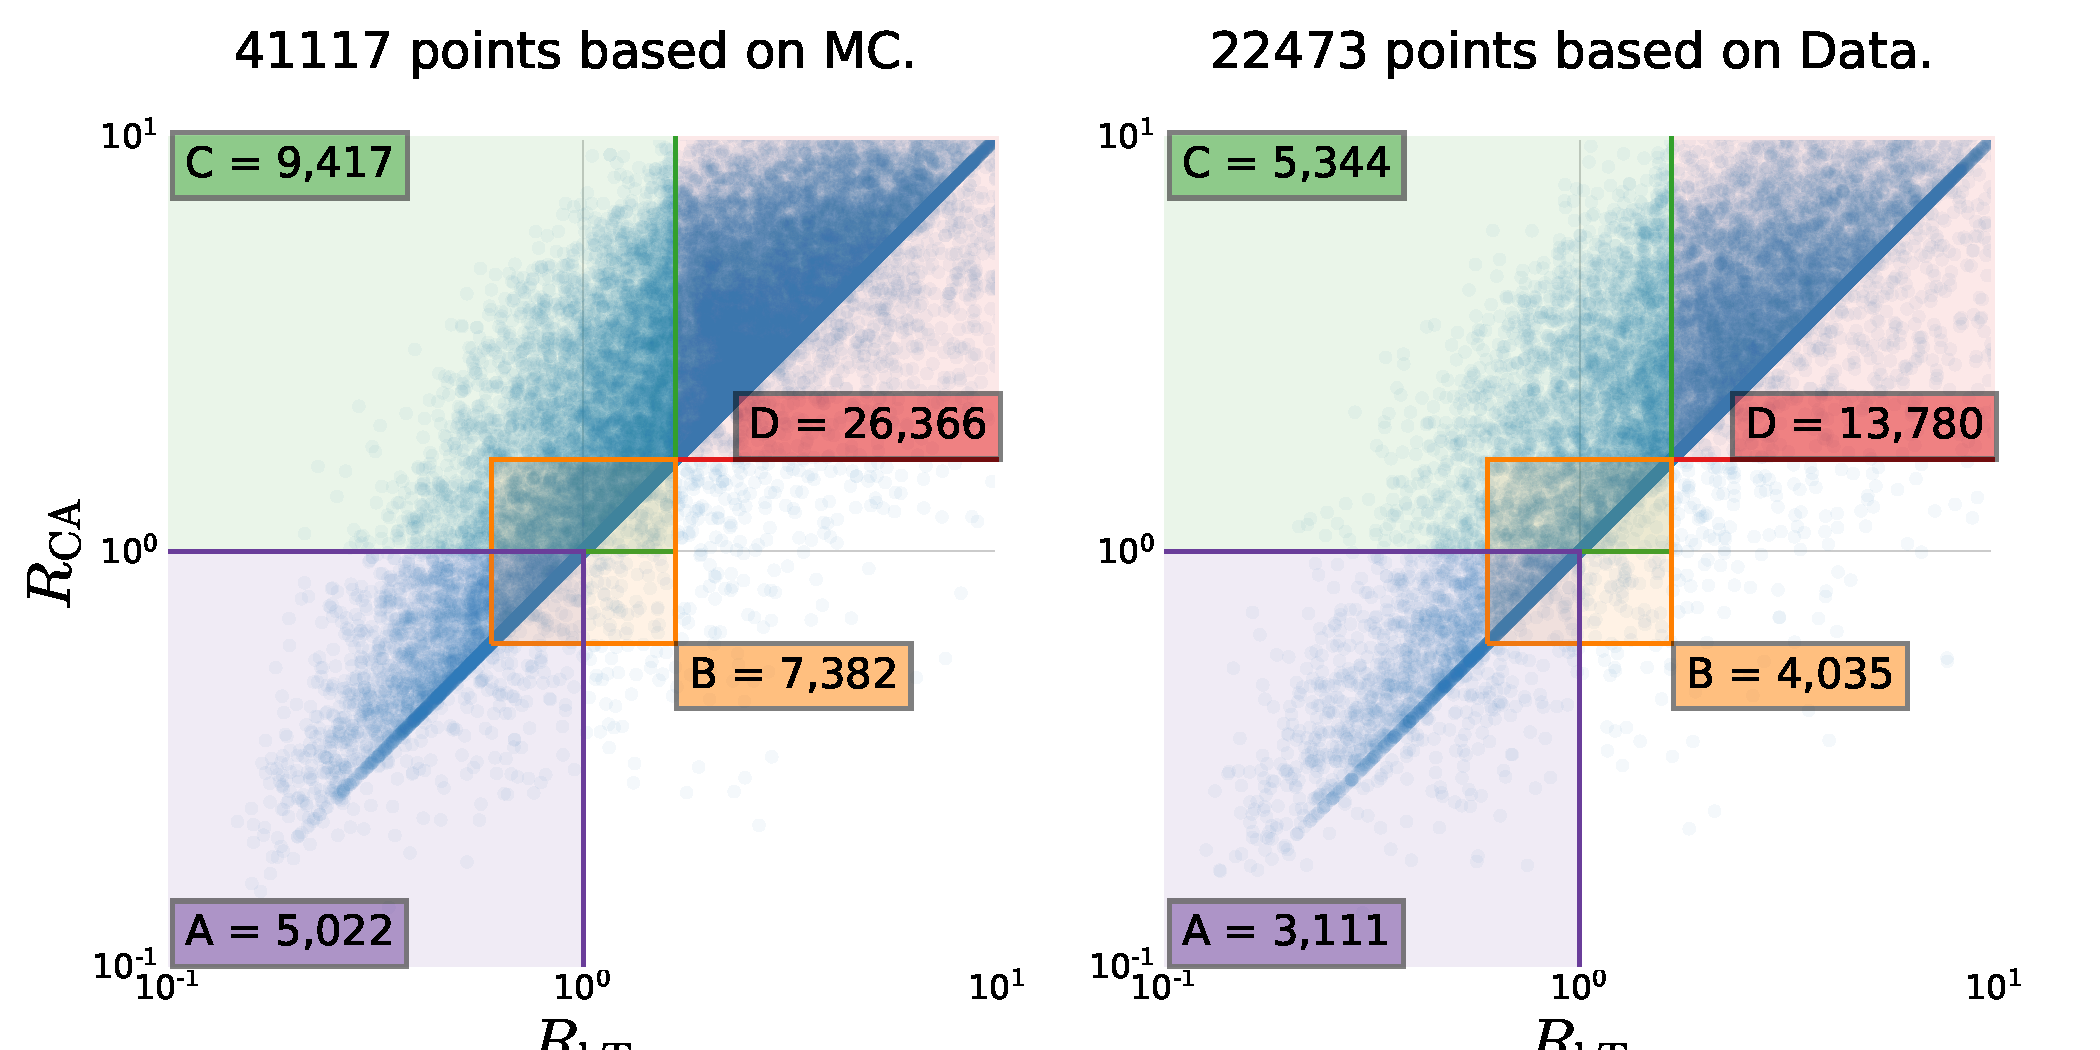
\includegraphics[width=0.95\textwidth, trim=0 0 0 118, clip, page=1]{figures/quarks/gtag-R_kt_CA_overview-down_sample=1.00-ML_vars=vertex-selection=b-ejet_min=4-n_iter_RS_lgb=99-n_iter_RS_xgb=9-cdot_cut=0.90-version=19-njet=4}
  \caption[R kt CA overview  XXX \TODO]
          {R kt CA overview XXX \TODO
          } 
  \label{fig:q:R_kt_CA_overview}
\end{figure}

\begin{figure}
  \includegraphics[width=0.95\textwidth, trim=0 0 0 30, clip, page=2]{figures/quarks/gtag-R_kt_CA_overview-down_sample=1.00-ML_vars=vertex-selection=b-ejet_min=4-n_iter_RS_lgb=99-n_iter_RS_xgb=9-cdot_cut=0.90-version=19-njet=4}
  \caption[R kt CA cut region A  XXX \TODO]
          {R kt CA cut region A XXX \TODO
          } 
  \label{fig:q:R_kt_CA_cut_A}
\end{figure}
